% -----------------------------------
% -------- BAYSIS - Matched ---------
% -----------------------------------
\subsection{Congestion - Accidents in general}
\label{analysis_processing_correlation_baysis_matched}
The correlation matrix table for the complete congestion-accident matched dataset (see \cref{table:appendix_correlation_matrix_matched_cramers}) is visual presented in \cref{img:correlation_matrix_matched_cramers} showing the the correlation of each variable combination. When visual analyzing \cref{img:correlation_matrix_matched_cramers} and checking the guidelines for a strong correlation in reference to the applied coefficient (identifiable with \cref{table:appendix_coefficient_matrix_matched}) we get a list of strongly correlated variable combinations (see \cref{tbl:correlation_list_baysis_matched}). Since the focus of the thesis are the correlations between accidents and jams, these are only collected from the bottom-left corner of the matrix, where the congestion and accidents variables intersect. Correlations of the kind congestion - congestion or accident - accident are not considered.
\begin{table}[ht!]
	\centering
	\begin{tabular}{c|l}  
		\toprule
		Category & Strong \\
		\midrule
		Str & TMax, TAvg, SMax, SAvg, TDist, SDist, Cov \\ 
 		Kat & TMax, TAvg, SAvg, TDist \\
 		Typ & TDist, Cov \\
 		%Betei & & \\
 		UArt1 & SAvg, TDist, Cov \\ % + SMax
 		%UArt2 & & \\
 		AUrs1 & SAvg, TDist, SDist, Cov, TLHGV \\ % + SMax
 		%AUrs2 & & \\
 		AufHi & TMax, TAvg, TDist, Cov \\
 		%Alkoh & & \\
 		%Char1 & & \\ % -> Strasse
 		%Char2 & & \\
 		%Bes1 & & \\
 		Lich1 & Cov \\
 		Lich2 & Cov \\ % + Lich2
 		Zust1 & Cov \\ % % -> Strasse
 		%Zust2 & & \\
 		%Fstf & & \\ % -> Strasse
 		WoTag & Cov \\
 		%FeiTag & & \\
		Month & Cov \\ % + TMax. SMAx
		\bottomrule
	\end{tabular}
	\caption{List of incident variables and their strong correlated congestion variable from the congestion-accident matched data}
	\label{tbl:correlation_list_baysis_matched}
\end{table}
Next we need to verify that the correlation is significant and what the correlation predicates. Therefore each correlation will be evaluated with the Post Hoc test, defined in \cref{correlation_posthoc}. \secintroend{baysis}{matched}
\begin{figure}[!ht]
	\centering
	\makebox[\textwidth][c]{%
		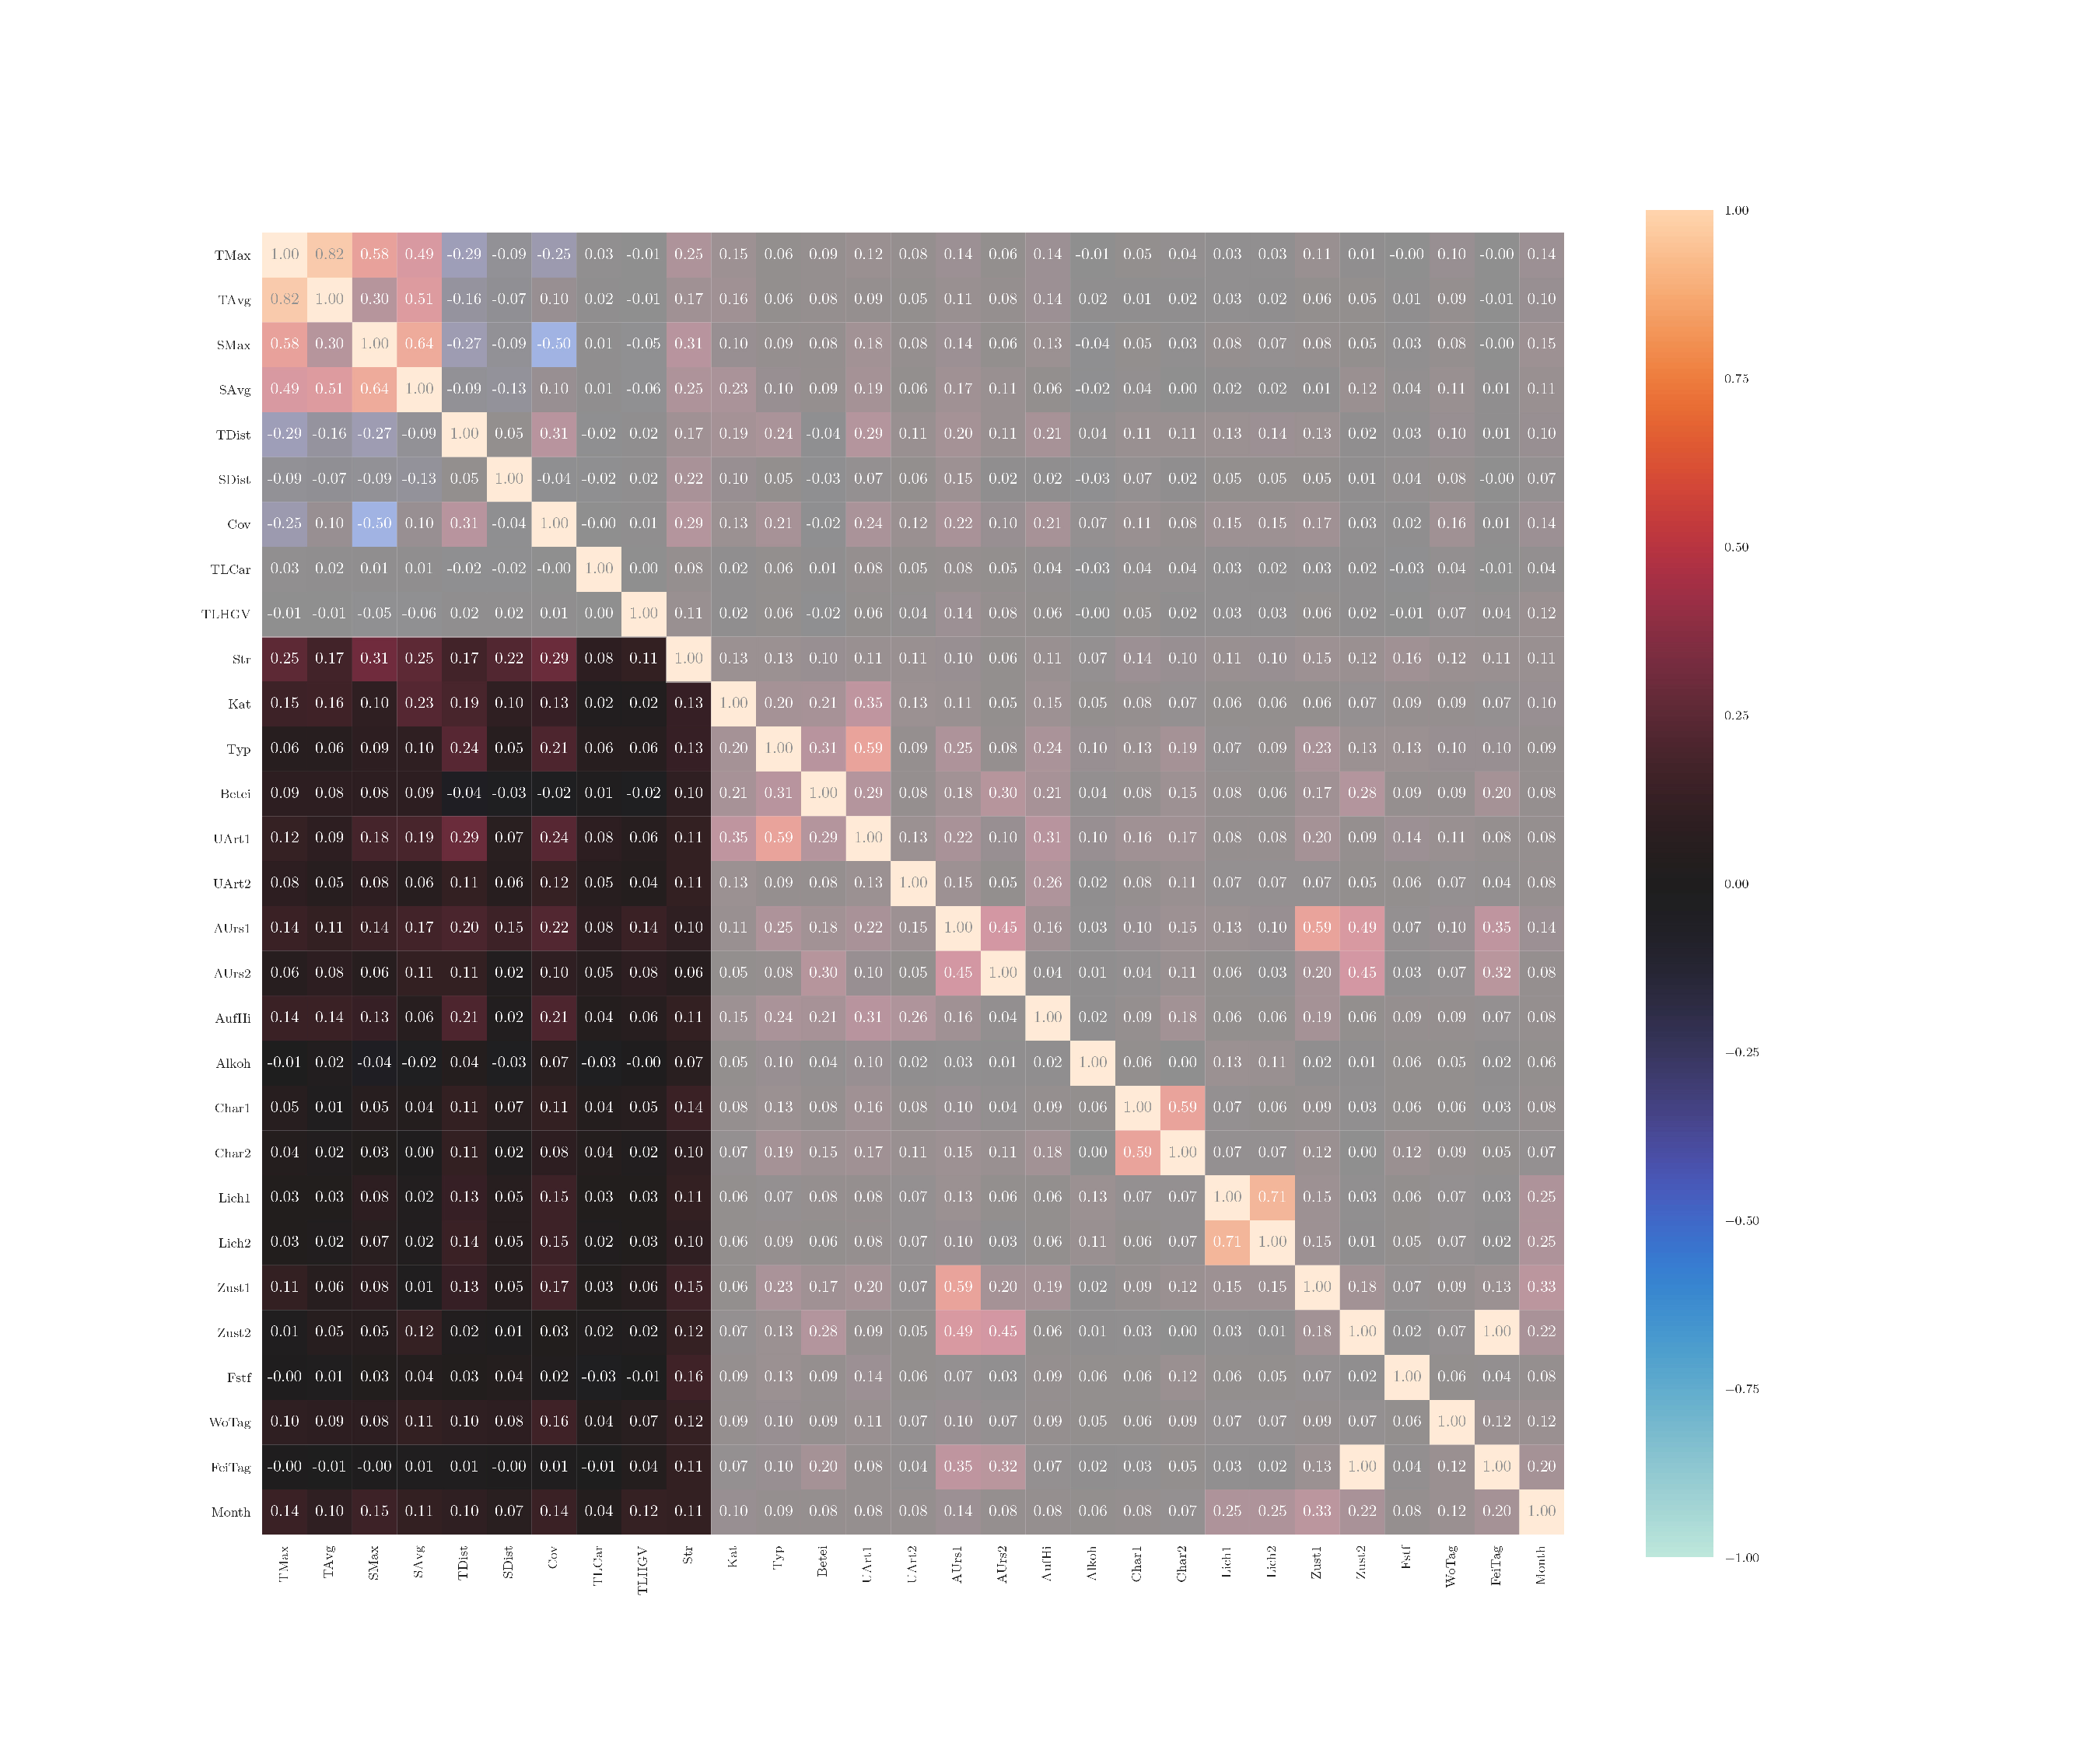
\includegraphics[width=1.4\textwidth, trim=0cm 2.5cm 6cm 3cm]{code/data/BAYSIS/02_matched/plots/baysis_matched_corr_cramers_edited}%
	}
	\caption{Correlation matrix for congestion-accident matched data calculated with $V$, $\eta$, $\tau$, $r_{pq}$, $r$}
	\label{img:correlation_matrix_matched_cramers}
\end{figure}

% --------------------------
% -------- Strasse ---------
% --------------------------
\centerheading{Street}
\label{ana:baysis_matched_Str}
\varintrosimplewithsam{Str}
\varintronosigmul{Str}{\textit{Str} - \textit{TDist} and \textit{Str} - \textit{SDist}}

% ##############################################
\groupintrosigsig{Str}{TMax}{baysis}{matched}
\begin{table}[ht!]
	\tiny
	\setlength{\tabcolsep}{4pt}
	\centering
	\begin{tabular}{rrrrrrrrrrrrrrrrr}
		\toprule
				& A3 & A6 & A9 & A70 & A96 & A7 & A73 & A99 & A92 & A93 & A94 & A72 & A995 & A95 & A71 & A45 \\ 
		\midrule
		% A6 		& 0.00 &  &  &  &  &  &  &  &  &  &  &  &  &  &  &  \\ 
		A9 		& \red{0.01} & 1.00 &  &  &  &  &  &  &  &  &  &  &  &  &  &  \\ 
		A70 	& \red{0.03} & 1.00 & 1.00 &  &  &  &  &  &  &  &  &  &  &  &  &  \\ 
		A96 	& \red{0.00} & 1.00 & 0.27 & 1.00 &  &  &  &  &  &  &  &  &  &  &  &  \\ 
		A7 		& \red{0.00} & 1.00 & 1.00 & 1.00 & 1.00 &  &  &  &  &  &  &  &  &  &  &  \\ 
		A73 	& \red{0.00} & 1.00 & 0.31 & 1.00 & 1.00 & 1.00 &  &  &  &  &  &  &  &  &  &  \\ 
		% A99 	& 1.00 & 1.00 & 1.00 & 1.00 & 0.50 & 1.00 & 0.59 &  &  &  &  &  &  &  &  &  \\ 
		A92 	& \red{0.00} & 1.00 & 0.16 & 1.00 & 1.00 & 1.00 & 1.00 & 0.22 &  &  &  &  &  &  &  &  \\ 
		% A93 	& 1.00 & 1.00 & 1.00 & 1.00 & 1.00 & 1.00 & 1.00 & 1.00 & 1.00 &  &  &  &  &  &  &  \\ 
		A94 	& \red{0.01} & 1.00 & 1.00 & 1.00 & 1.00 & 1.00 & 1.00 & 1.00 & 1.00 & 1.00 &  &  &  &  &  &  \\ 
		% A72 	& 1.00 & 1.00 & 1.00 & 1.00 & 1.00 & 1.00 & 1.00 & 1.00 & 1.00 & 1.00 & 1.00 &  &  &  &  &  \\ 
		% A995 	& 1.00 & 1.00 & 1.00 & 1.00 & 1.00 & 1.00 & 1.00 & 1.00 & 1.00 & 1.00 & 1.00 & 1.00 &  &  &  &  \\ 
		% A95 	& 1.00 & 1.00 & 1.00 & 1.00 & 1.00 & 1.00 & 1.00 & 1.00 & 1.00 & 1.00 & 1.00 & 1.00 & 1.00 &  &  &  \\ 
		% A71 	& 1.00 & 1.00 & 1.00 & 1.00 & 1.00 & 1.00 & 1.00 & 1.00 & 1.00 & 1.00 & 1.00 & 1.00 & 1.00 & 1.00 &  &  \\ 
		% A45 	& 1.00 & 1.00 & 1.00 & 1.00 & 1.00 & 1.00 & 1.00 & 1.00 & 1.00 & 1.00 & 1.00 & 1.00 & 1.00 & 1.00 & 1.00 &  \\ 
		% A980 	& 1.00 & 1.00 & 1.00 & 1.00 & 1.00 & 1.00 & 1.00 & 1.00 & 1.00 & 1.00 & 1.00 & 1.00 & 1.00 & 1.00 & 1.00 & 1.00 \\ 
		\bottomrule
	\end{tabular}
	\caption{Pairwise Wilcoxon $T$-test for \textit{Street} and \textit{Maximal Temporal Extent}, see \cref{tbl:wilcoxon_baysis_matched_Str_TMax_complete} for complete table}
	\label{tbl:wilcoxon_baysis_matched_Str_TMax}
\end{table}
It shows that the groups A6, A9, A7, A70, A73, A92, A94 and A96 differ significantly from group A3, but there is no distinctive general trend.
% #### START: Table and Plot
\begin{figure}[ht!]
	\centering
	\begin{minipage}{0.5\textwidth}
		\tiny
		\setlength{\tabcolsep}{4pt}
		\centering
		\begin{tabular}{c|c|c|c|c|c|c|c}
			\toprule
			Group & $n$ & $\bar{x}$ & $\sigma$ & $\tilde{x}$ & $min$ & $max$ & $\Delta$ \\
			\midrule
			A3  & 559 & 225.76 & 210.36 & 156.0 & 9  & 1323 & 1314 \\ 
			A6  & 127 & 153.05 & 150.42 & 108.0 & 12 & 864  & 852  \\ 
			A9  & 466 & 170.85 & 151.33 & 118.5 & 9  & 1194 & 1185 \\ 
			A70 & 31  & 106.55 & 79.42  & 81.0 & 24 & 369  & 345  \\ 
			A96 & 155 & 118.32 & 81.05  & 108.0 & 12 & 384  & 372  \\ 
			A7  & 130 & 153.37 & 194.10 & 102.0 & 9  & 1341 & 1332 \\ 
			A73 & 129 & 125.95 & 135.01 & 93.0 & 12 & 1323 & 1311 \\ 
			A99 & 116 & 169.09 & 136.72 & 138.0 & 15 & 681  & 666  \\ 
			A92 & 66  & 103.86 & 65.69  & 87.0 & 18 & 354  & 336  \\ 
			A93 & 21  & 163.57 & 155.71 & 111.0 & 36 & 588  & 552  \\ 
			A94 & 37  & 101.59 & 54.60  & 99.0 & 15 & 249  & 234  \\ 
			\bottomrule
			% \bar{x} - sum = 1591.96, mean = 144.72
			% \sigma - sum = 1414.41, mean = 128.58
			% \tilde{x}
		\end{tabular}
		\subcaption[second caption.]{Table of all descriptives}\label{tbl:descriptives_baysis_matched_Str_TMax}
	\end{minipage}%
	\begin{minipage}{0.55\textwidth}
		\pgfplotstableread[col sep=comma]{
			road, count, mean, median, sd, min, max, delta
			A3  , 559 , 225.76 , 210.36 , 156.0 , 9  , 1323 , 1314 
			A6  , 127 , 153.05 , 150.42 , 108.0 , 12 , 864  , 852  
			A9  , 466 , 170.85 , 151.33 , 118.5 , 9  , 1194 , 1185 
			A70 , 31  , 106.55 , 79.42  , 81.0  , 24 , 369  , 345  
			A96 , 155 , 118.32 , 81.05  , 108.0 , 12 , 384  , 372  
			A7  , 130 , 153.37 , 194.10 , 102.0 , 9  , 1341 , 1332 
			A73 , 129 , 125.95 , 135.01 , 93.0  , 12 , 1323 , 1311 
			A99 , 116 , 169.09 , 136.72 , 138.0 , 15 , 681  , 666  
			A92 , 66  , 103.86 , 65.69  , 87.0  , 18 , 354  , 336  
			A93 , 21  , 163.57 , 155.71 , 111.0 , 36 , 588  , 552  
			A94 , 37  , 101.59 , 54.60  , 99.0  , 15 , 249  , 234  
		}\data
		\pgfplotstablesort[sort key=mean, sort cmp=float >]{\datasorted}{\data}
		\tiny
		\centering
		\descplotfigwithavg{\datasorted}{144}{128}{10}{4.7}
		\subcaption[second caption.]{Plot of descriptives $\bar{x}$, $\sigma$ and $\tilde{x}$}\label{fig:descriptives_baysis_matched_Str_TMax}
	\end{minipage}%
	\caption{Group descriptives of \textit{Street} and \textit{Maximal Temporal Extent}}
	%\vspace{-8mm}
\end{figure}
% #### END: Table and Plot
The significant descriptives from \cref{tbl:descriptives_baysis_matched_Str_TMax,fig:descriptives_baysis_matched_Str_TMax} show that the $\bar{x}$ duration of the A3 is 72\,min - 154\,min higher than the $\bar{x}$ of A6, A7, A9, A70, A73, A92, and A94. Therefore it can be interpreted that accidents on the A3 are associated with significantly longer (temporal) jams than on the A6, A9, A7, A70, A73, A92, and A94. The descriptives also show that the A70, A73, A92, A94 and A96 are have considerable shorter durations, when the A3, A9 and A99 have considerable longer duration compared to the overall $\bar{x}$.
\groupintrosig{Str}{TAvg}{0.0004}{baysis}{matched}
\begin{table}[ht!]
	\tiny
	\setlength{\tabcolsep}{4pt}
	\centering
	\begin{tabular}{rrrrrrrrrrrrrrrrr}
		\toprule
				& A3 & A6 & A9 & A70 & A96 & A7 & A73 & A99 & A92 & A93 & A94 & A72 & A995 & A95 & A71 & A45 \\ 
		\midrule
		% A6 	 & 0.84 &  &  &  &  &  &  &  &  &  &  &  &  &  &  &  \\ 
		% A9 	 & 0.36 & 1.00 &  &  &  &  &  &  &  &  &  &  &  &  &  &  \\ 
		% A70	 & 1.00 & 1.00 & 1.00 &  &  &  &  &  &  &  &  &  &  &  &  &  \\ 
		% A96  & 0.10 & 1.00 & 1.00 & 1.00 &  &  &  &  &  &  &  &  &  &  &  &  \\ 
		% A7 	 & 1.00 & 1.00 & 1.00 & 1.00 & 1.00 &  &  &  &  &  &  &  &  &  &  &  \\ 
		A73  & \red{0.00} & 1.00 & 0.51 & 1.00 & 1.00 & 1.00 &  &  &  &  &  &  &  &  &  &  \\ 
		A99  & \red{0.02} & 1.00 & 1.00 & 1.00 & 1.00 & 1.00 & 1.00 &  &  &  &  &  &  &  &  &  \\ 
		% A92  & 0.26 & 1.00 & 1.00 & 1.00 & 1.00 & 1.00 & 1.00 & 1.00 &  &  &  &  &  &  &  &  \\ 
		% A93  & 1.00 & 1.00 & 1.00 & 1.00 & 1.00 & 1.00 & 1.00 & 1.00 & 1.00 &  &  &  &  &  &  &  \\ 
		% A94  & 0.28 & 1.00 & 1.00 & 1.00 & 1.00 & 1.00 & 1.00 & 1.00 & 1.00 & 1.00 &  &  &  &  &  &  \\ 
		% A72  & 1.00 & 1.00 & 1.00 & 1.00 & 1.00 & 1.00 & 1.00 & 1.00 & 1.00 & 1.00 & 1.00 &  &  &  &  &  \\ 
		% A995 & 1.00 & 1.00 & 1.00 & 1.00 & 1.00 & 1.00 & 1.00 & 1.00 & 1.00 & 1.00 & 1.00 & 1.00 &  &  &  &  \\ 
		% A95  & 1.00 & 1.00 & 1.00 & 1.00 & 1.00 & 1.00 & 1.00 & 1.00 & 1.00 & 1.00 & 1.00 & 1.00 & 1.00 &  &  &  \\ 
		% A71	 & 1.00 & 1.00 & 1.00 & 1.00 & 1.00 & 1.00 & 1.00 & 1.00 & 1.00 & 1.00 & 1.00 & 1.00 & 1.00 & 1.00 &  &  \\ 
		% A45  & 1.00 & 1.00 & 1.00 & 1.00 & 1.00 & 1.00 & 1.00 & 1.00 & 1.00 & 1.00 & 1.00 & 1.00 & 1.00 & 1.00 & 1.00 &  \\ 
		% A980 & 1.00 & 1.00 & 1.00 & 1.00 & 1.00 & 1.00 & 1.00 & 1.00 & 1.00 & 1.00 & 1.00 & 1.00 & 1.00 & 1.00 & 1.00 & 1.00 \\
		\bottomrule
	\end{tabular}
	\caption{Pairwise Wilcoxon $T$-test for \textit{Street} and \textit{Average Temporal Extent}, see \cref{tbl:wilcoxon_baysis_matched_Str_TAvg_complete} for complete table}
	\label{tbl:wilcoxon_baysis_matched_Str_TAvg}
\end{table}
The table shows that just the groups A73 and A99 differ significantly from group A3, but there is no distinctive general trend.
% #### START: Table and Plot
\begin{figure}[ht!]
	\centering
	\begin{minipage}{0.5\textwidth}
		\tiny
		\setlength{\tabcolsep}{4pt}
		\centering
		\begin{tabular}{c|c|c|c|c|c|c|c}
			\toprule
			Group & $n$ & $\bar{x}$ & $\sigma$ & $\tilde{x}$ & $min$ & $max$ & $\Delta$ \\
			\midrule
			A3  & 559 & 89.66 & 98.94  & 65.00 & 4  & 1260 & 1256 \\ 
			A6  & 127 & 69.94 & 65.86  & 56.00 & 3  & 376  & 373  \\ 
			A9  & 466 & 72.92 & 64.55  & 54.00 & 4  & 575  & 571  \\ 
			A70 & 31  & 50.10 & 23.99  & 49.00 & 10 & 99   & 89   \\ 
			A96 & 155 & 61.37 & 44.31  & 52.50 & 5  & 247  & 242  \\ 
			A7  & 130 & 86.55 & 146.82 & 59.50 & 6  & 1326 & 1320 \\ 
			A73 & 129 & 54.78 & 42.48  & 45.00 & 6  & 274  & 268  \\ 
			A99 & 116 & 58.97 & 48.35  & 47.50 & 4  & 295  & 291  \\ 
			A92 & 66  & 55.24 & 36.43  & 51.50 & 8  & 235  & 227  \\ 
			A93 & 21  & 82.33 & 91.10  & 48.00 & 7  & 343  & 336  \\ 
			A94 & 37  & 49.86 & 31.63  & 44.00 & 14 & 145  & 131  \\ 
			\bottomrule
			% \bar{x} - sum = 731.72, mean = 66.52
			% \sigma - sum = 694.46, mean = 63.13
			% \tilde{x}
		\end{tabular}
		\subcaption[second caption.]{Table of all descriptives}\label{tbl:descriptives_baysis_matched_Str_TAvg}
	\end{minipage}%
	\begin{minipage}{0.55\textwidth}
		\pgfplotstableread[col sep=comma]{
			road, count, mean, median, sd, min, max, delta
			A3  , 559 , 89.66 , 98.94  , 65.00 , 4  , 1260 , 1256 
			A6  , 127 , 69.94 , 65.86  , 56.00 , 3  , 376  , 373  
			A9  , 466 , 72.92 , 64.55  , 54.00 , 4  , 575  , 571  
			A70 , 31  , 50.10 , 23.99  , 49.00 , 10 , 99   , 89   
			A96 , 155 , 61.37 , 44.31  , 52.50 , 5  , 247  , 242  
			A7  , 130 , 86.55 , 146.82 , 59.50 , 6  , 1326 , 1320 
			A73 , 129 , 54.78 , 42.48  , 45.00 , 6  , 274  , 268  
			A99 , 116 , 58.97 , 48.35  , 47.50 , 4  , 295  , 291  
			A92 , 66  , 55.24 , 36.43  , 51.50 , 8  , 235  , 227  
			A93 , 21  , 82.33 , 91.10  , 48.00 , 7  , 343  , 336  
			A94 , 37  , 49.86 , 31.63  , 44.00 , 14 , 145  , 131   
		}\data
		\pgfplotstablesort[sort key=mean, sort cmp=float >]{\datasorted}{\data}
		\tiny
		\centering
		\descplotfigwithavg{\datasorted}{66}{63}{10}{4.7}
		\subcaption[second caption.]{Plot of descriptives $\bar{x}$, $\sigma$ and $\tilde{x}$}\label{fig:descriptives_baysis_matched_Str_TAvg}
	\end{minipage}%
	\caption{Group descriptives of \textit{Street} and \textit{Average Temporal Extent}}
	%\vspace{-8mm}
\end{figure}
% #### END: Table and Plot
The significant descriptives from \cref{tbl:descriptives_baysis_matched_Str_TAvg,fig:descriptives_baysis_matched_Str_TAvg} show that the $\bar{x}$ value of A3 is about 48\,min higher than the $\bar{x}$ of A73 and A96. Therefore it can be interpreted that accidents on the A3 are associated with significantly longer (temporal) jams than on the A73 and A96. The descriptives show also that the A3, A7, A9 and A93 are have considerable shorter durations, when the A70, A73, A92, and A94 have considerable longer duration compared to the overall $\bar{x}$.
\begin{figure}[ht!]
	\pgfplotstableread[col sep=comma]{
		Road, meanTMax, meanTAvg
		A3  , 225.76 , 89.66  
		A6  , 153.05 , 69.94  
		A9  , 170.85 , 72.92  
		A70 , 106.55 , 50.10  
		A96 , 118.32 , 61.37  
		A7  , 153.37 , 86.55  
		A73 , 125.95 , 54.78  
		A99 , 169.09 , 58.97  
		A92 , 103.86 , 55.24  
		A93 , 163.57 , 82.33  
		A94 , 101.59 , 49.86    
	}\data
	\pgfplotstablesort[sort key=meanTAvg, sort cmp=float >]{\datasorted}{\data}
	\tiny
	\centering
	\barplotdouble{\datasorted}{meanTMax}{meanTAvg}{$\bar{x}_{TMax}$}{$\bar{x}_{TAvg}$}
	\caption{Comparison of descriptives $\bar{x}_{TMax}$ and $\bar{x}_{TAvg}$ (\textit{TMax/TAvg} by \textit{Street})}
	\label{fig:baysis_matched_meancomparison_Str_temporal}
	%\vspace{-8mm}
\end{figure}
When comparing the $\bar{x}$ values of the maximal and average (temporal) extend (shown in \cref{fig:baysis_matched_meancomparison_Str_temporal}) it becomes clear that the average variable has considerable lower values than the maximum variable, which is to be expected. It also shows, that the differences between the groups are mostly similar in both the maximal and average extend, but vary considerably. In can be described that the follow the same tend. This trend is especially ignored by the A99, which probably means that there are more errors in the maximal (temporal) extend variable on the A99.

% ##############################################
\groupintrosigsig{Str}{SMax}{baysis}{matched}
\begin{table}[ht!]
	\tiny
	\setlength{\tabcolsep}{4pt}
	\centering
	\begin{tabular}{rrrrrrrrrrrrrrrrr}
		\toprule
				& A3   & A6   & A9   & A70  & A96  & A7   & A73   & A99 & A92 & A93 & A94 & A72 & A995 & A95 & A71 & A45 \\ 
		\midrule
		% A6 		& 0.40 &  &  &  &  &  &  &  &  &  &  &  &  &  &  &  \\ 
		A9 		& \red{0.00} & 1.00 &  &  &  &  &  &  &  &  &  &  &  &  &  &  \\ 
		A70 	& \red{0.00} & 0.83 & 0.54 &  &  &  &  &  &  &  &  &  &  &  &  &  \\ 
		A96 	& \red{0.00} & 1.00 & 0.14 & 1.00 &  &  &  &  &  &  &  &  &  &  &  &  \\ 
		A7 		& \red{0.00} & 1.00 & 1.00 & 1.00 & 1.00 &  &  &  &  &  &  &  &  &  &  &  \\ 
		A73 	& \red{0.00} & \red{0.00} & \red{0.00} & 1.00 & 1.00 & 0.59 &  &  &  &  &  &  &  &  &  &  \\ 
		A99 	& 1.00 & 1.00 & 1.00 & 0.80 & 0.31 & 1.00 & \red{0.00} &  &  &  &  &  &  &  &  &  \\ 
		A92 	& \red{0.00} & \red{0.00} & \red{0.00} & 1.00 & 1.00 & 1.00 & 1.00 & \red{0.00} &  &  &  &  &  &  &  &  \\ 
		A93 	& \red{0.03} & 1.00 & 1.00 & 1.00 & 1.00 & 1.00 & 1.00 & 1.00 & 1.00 &  &  &  &  &  &  &  \\ 
		A94 	& \red{0.00} & 0.11 & \red{0.03} & 1.00 & 1.00 & 1.00 & 1.00 & 0.09 & 1.00 & 1.00 &  &  &  &  &  &  \\ 
		% A72 	& 1.00 & 1.00 & 1.00 & 1.00 & 1.00 & 1.00 & 1.00 & 1.00 & 1.00 & 1.00 & 1.00 &  &  &  &  &  \\ 
		% A995 	& 1.00 & 1.00 & 1.00 & 1.00 & 1.00 & 1.00 & 1.00 & 1.00 & 1.00 & 1.00 & 1.00 & 1.00 &  &  &  &  \\ 
		% A95 	& 1.00 & 1.00 & 1.00 & 1.00 & 1.00 & 1.00 & 1.00 & 1.00 & 1.00 & 1.00 & 1.00 & 1.00 & 1.00 &  &  &  \\ 
		% A71 	& 1.00 & 1.00 & 1.00 & 1.00 & 1.00 & 1.00 & 1.00 & 1.00 & 1.00 & 1.00 & 1.00 & 1.00 & 1.00 & 1.00 &  &  \\ 
		% A45 	& 1.00 & 1.00 & 1.00 & 1.00 & 1.00 & 1.00 & 1.00 & 1.00 & 1.00 & 1.00 & 1.00 & 1.00 & 1.00 & 1.00 & 1.00 &  \\ 
		% A980 	& 1.00 & 1.00 & 1.00 & 1.00 & 1.00 & 1.00 & 1.00 & 1.00 & 1.00 & 1.00 & 1.00 & 1.00 & 1.00 & 1.00 & 1.00 & 1.00 \\ 
		\bottomrule
	\end{tabular}
	\caption{Pairwise Wilcoxon $T$-test for \textit{Street} and \textit{Maximal Spatial Extent}, see \cref{tbl:wilcoxon_baysis_matched_Str_SMax_complete} for complete table}
	\label{tbl:wilcoxon_baysis_matched_Str_SMax}
\end{table}
It shows, that the groups A7, A9, A70, A73, A92, A94 and A96 differ significantly from group A3. The groups A73 and A92 further differ significantly from group A6 and A9. The group A99 differs significantly from group A73 and group A92 differs from A99, but there is no distinctive general trend.
% #### START: Table and Plot
\begin{figure}[ht!]
	\centering
	\begin{minipage}{0.5\textwidth}
		\tiny
		\setlength{\tabcolsep}{4pt}
		\centering
		\begin{tabular}{c|c|c|c|c|c|c|c}
			\toprule
			Group & $n$ & $\bar{x}$ & $\sigma$ & $\tilde{x}$ & $min$ & $max$ & $\Delta$ \\
			\midrule
			A3  & 559 & 13874.96 & 10064.51 & 11014.00 & 1084 & 46328 & 45244 \\ 
			A6  & 127 & 11067.98 & 8428.07  & 8634.00  & 965  & 43156 & 42191 \\ 
			A9  & 466 & 10680.48 & 7724.45  & 8977.50  & 832  & 49765 & 48933 \\ 
			A70 & 31  & 6676.39  & 3640.24  & 6136.00  & 1841 & 13058 & 11217 \\ 
			A96 & 155 & 8551.75  & 6431.18  & 6238.00  & 971  & 27965 & 26994 \\ 
			A7  & 130 & 9018.27  & 7293.14  & 7051.50  & 1108 & 43244 & 42136 \\ 
			A73 & 129 & 6502.88  & 5033.20  & 5327.00  & 1036 & 33764 & 32728 \\ 
			A99 & 116 & 13244.02 & 11313.27 & 9439.50  & 1280 & 48278 & 46998 \\ 
			A92 & 66  & 6186.80  & 4000.10  & 4936.50  & 1176 & 23291 & 22115 \\ 
			A93 & 21  & 6765.00  & 4403.32  & 5323.00  & 1244 & 16922 & 15678 \\ 
			A94 & 37  & 6220.38  & 3984.46  & 5768.00  & 1167 & 15550 & 14383 \\ 
			\bottomrule
			% \bar{x} - sum = 98788.91, mean = 8980.81
			% \sigma - sum = 72315.94, mean = 6574.17
			% \tilde{x}
		\end{tabular}
		\subcaption[second caption.]{Table of all descriptives}\label{tbl:descriptives_baysis_matched_Str_SMax}
	\end{minipage}%
	\begin{minipage}{0.55\textwidth}
		\pgfplotstableread[col sep=comma]{
			road, count, mean, median, sd, min, max, delta
			A3  , 559 , 13874.96 , 10064.51 , 11014.00 , 1084 , 46328 , 45244 
			A6  , 127 , 11067.98 , 8428.07  , 8634.00  , 965  , 43156 , 42191 
			A9  , 466 , 10680.48 , 7724.45  , 8977.50  , 832  , 49765 , 48933 
			A70 , 31  , 6676.39  , 3640.24  , 6136.00  , 1841 , 13058 , 11217 
			A96 , 155 , 8551.75  , 6431.18  , 6238.00  , 971  , 27965 , 26994 
			A7  , 130 , 9018.27  , 7293.14  , 7051.50  , 1108 , 43244 , 42136 
			A73 , 129 , 6502.88  , 5033.20  , 5327.00  , 1036 , 33764 , 32728 
			A99 , 116 , 13244.02 , 11313.27 , 9439.50  , 1280 , 48278 , 46998 
			A92 , 66  , 6186.80  , 4000.10  , 4936.50  , 1176 , 23291 , 22115 
			A93 , 21  , 6765.00  , 4403.32  , 5323.00  , 1244 , 16922 , 15678 
			A94 , 37  , 6220.38  , 3984.46  , 5768.00  , 1167 , 15550 , 14383   
		}\data
		\pgfplotstablesort[sort key=mean, sort cmp=float >]{\datasorted}{\data}
		\tiny
		\centering
		\descplotfigwithcustomavg{\datasorted}{8980}{6574}{0.89}{0.65}{10}{4.7}
		\subcaption[second caption.]{Plot of descriptives $\bar{x}$, $\sigma$ and $\tilde{x}$}\label{fig:descriptives_baysis_matched_Str_SMax}
	\end{minipage}%
	\caption{Group descriptives of \textit{Street} and \textit{Maximal Spatial Extent}}
	%\vspace{-8mm}
\end{figure}
% #### END: Table and Plot
The significant descriptives from \cref{tbl:descriptives_baysis_matched_Str_SMax,fig:descriptives_baysis_matched_Str_SMax} show that the $\bar{x}$ of A3 is 3194\,m - 7688\,m higher than the $\bar{x}$ of A7, A9, A70, A73, A92, A94 and A96. They also shows that the groups A6, A9 and A99 have a 5163\,m higher $\bar{x}$ on average than the groups A73 and A92. Therefore it can be interpreted that accidents on the A3, A6, A9 and A99 are associated with significantly longer (spatial) jams than on A7, A73, A92, A94 and A96. The descriptives show also that the A3, A6 A9 and A99 have a considerable longer lengths, when the A70, A73, A92, A93 and A94 have considerable shorter lengths compared to the overall $\bar{x}$.
\groupintrosig{Str}{SAvg}{0.0027}{baysis}{matched}
\begin{table}[ht!]
	\tiny
	\setlength{\tabcolsep}{4pt}
	\centering
	\begin{tabular}{rrrrrrrrrrrrrrrrr}
		\toprule
	 		 & A3 & A6 & A9 & A70 & A96 & A7 & A73 & A99 & A92 & A93 & A94 & A72 & A995 & A95 & A71 & A45 \\ 
		\midrule
		% A6   & 1.00 &  &  &  &  &  &  &  &  &  &  &  &  &  &  &  \\ 
	  	% A9   & 1.00 & 1.00 &  &  &  &  &  &  &  &  &  &  &  &  &  &  \\ 
	  	A70  & \red{0.05} & 0.83 & 0.71 &  &  &  &  &  &  &  &  &  &  &  &  &  \\ 
	  	A96  & \red{0.05} & 1.00 & 1.00 & 1.00 &  &  &  &  &  &  &  &  &  &  &  &  \\ 
	  	% A7   & 1.00 & 1.00 & 1.00 & 1.00 & 1.00 &  &  &  &  &  &  &  &  &  &  &  \\ 
	  	A73  & \red{0.00} & \red{0.00} & \red{0.00} & 1.00 & \red{0.00} & \red{0.00} &  &  &  &  &  &  &  &  &  &  \\ 
	  	A99  & \red{0.00} & 1.00 & 0.06 & 1.00 & 1.00 & 1.00 & 0.51 &  &  &  &  &  &  &  &  &  \\ 
	  	A92  & \red{0.00} & 0.61 & \red{0.03} & 1.00 & 1.00 & 1.00 & 1.00 & 1.00 &  &  &  &  &  &  &  &  \\ 
	  	A93  & \red{0.03} & 0.46 & 0.16 & 1.00 & 1.00 & 1.00 & 1.00 & 1.00 & 1.00 &  &  &  &  &  &  &  \\ 
	  	A94  & \red{0.00} & 0.07 & 0.01 & 1.00 & 0.36 & 0.31 & 1.00 & 1.00 & 1.00 & 1.00 &  &  &  &  &  &  \\ 
	  	% A72  & 1.00 & 1.00 & 1.00 & 1.00 & 1.00 & 1.00 & 1.00 & 1.00 & 1.00 & 1.00 & 1.00 &  &  &  &  &  \\ 
	  	% A995 & 1.00 & 1.00 & 1.00 & 1.00 & 1.00 & 1.00 & 1.00 & 1.00 & 1.00 & 1.00 & 1.00 & 1.00 &  &  &  &  \\ 
	  	% A95  & 1.00 & 1.00 & 1.00 & 1.00 & 1.00 & 1.00 & 1.00 & 1.00 & 1.00 & 1.00 & 1.00 & 1.00 & 1.00 &  &  &  \\ 
	  	% A71  & 1.00 & 1.00 & 1.00 & 1.00 & 1.00 & 1.00 & 1.00 & 1.00 & 1.00 & 1.00 & 1.00 & 1.00 & 1.00 & 1.00 &  &  \\ 
	  	% A45  & 1.00 & 1.00 & 1.00 & 1.00 & 1.00 & 1.00 & 1.00 & 1.00 & 1.00 & 1.00 & 1.00 & 1.00 & 1.00 & 1.00 & 1.00 &  \\ 
	  	% A980 & 1.00 & 1.00 & 1.00 & 1.00 & 1.00 & 1.00 & 1.00 & 1.00 & 1.00 & 1.00 & 1.00 & 1.00 & 1.00 & 1.00 & 1.00 & 1.00 \\ 
		\bottomrule
	\end{tabular}
	\caption{Pairwise Wilcoxon $T$-test for \textit{Street} and \textit{Average Spatial Extent}, see \cref{tbl:wilcoxon_baysis_matched_Str_SAvg_complete} for complete table}
	\label{tbl:wilcoxon_baysis_matched_Str_SAvg}
\end{table}
It shows, that the groups A70, A73, A92, A93, A94, A96 and A99 differ significantly from group A3. The groups A73 further differ significantly from group A6, A7, A9 and A96. The A92 also differs significantly from group A9, but there is no distinctive general trend.
% #### START: Table and Plot
\begin{figure}[ht!]
	\centering
	\begin{minipage}{0.5\textwidth}
		\tiny
		\setlength{\tabcolsep}{4pt}
		\centering
		\begin{tabular}{c|c|c|c|c|c|c|c}
			\toprule
			Group & $n$ & $\bar{x}$ & $\sigma$ & $\tilde{x}$ & $min$ & $max$ & $\Delta$ \\
			\midrule
			A3  & 559 & 4537.56 & 2735.62 & 3986.0 & 135  & 17805 & 17670 \\ 
			A6  & 127 & 4361.50 & 3042.71 & 3235.0 & 458  & 16851 & 16393 \\ 
			A9  & 466 & 4187.15 & 2569.83 & 3700.5 & 393  & 15132 & 14739 \\ 
			A70 & 31  & 3010.45 & 2067.63 & 1974.0 & 1008 & 9937  & 8929 \\ 
			A96 & 155 & 3678.39 & 2172.99 & 3299.0 & 387  & 10182 & 9795 \\ 
			A7  & 130 & 4141.68 & 3026.58 & 3537.5 & 643  & 16571 & 15928 \\ 
			A73 & 129 & 2683.97 & 1981.91 & 2232.0 & 544  & 11832 & 11288 \\ 
			A99 & 116 & 3240.97 & 1878.87 & 2978.0 & 583  & 8426  & 7843 \\ 
			A92 & 66  & 2926.15 & 1521.59 & 2931.5 & 455  & 8970  & 8515 \\ 
			A93 & 21  & 2525.43 & 1443.21 & 2338.0 & 664  & 6779  & 6115 \\ 
			A94 & 37  & 2691.68 & 2023.38 & 2307.0 & 358  & 10393 & 10035 \\ 
			\bottomrule
			% \bar{x} - sum = 37984.93, mean = 3453.17
			% \sigma - sum = 24464.32, mean = 2224.02
			% \tilde{x}
		\end{tabular}
		\subcaption[second caption.]{Table of all descriptives}\label{tbl:descriptives_baysis_matched_Str_SAvg}
	\end{minipage}%
	\begin{minipage}{0.55\textwidth}
		\pgfplotstableread[col sep=comma]{
			road, count, mean, median, sd, min, max, delta
			A3  , 559 , 4537.56 , 2735.62 , 3986.0 , 135  , 17805 , 17670
			A6  , 127 , 4361.50 , 3042.71 , 3235.0 , 458  , 16851 , 16393
			A9  , 466 , 4187.15 , 2569.83 , 3700.5 , 393  , 15132 , 14739
			A70 , 31  , 3010.45 , 2067.63 , 1974.0 , 1008 , 9937  , 8929 
			A96 , 155 , 3678.39 , 2172.99 , 3299.0 , 387  , 10182 , 9795 
			A7  , 130 , 4141.68 , 3026.58 , 3537.5 , 643  , 16571 , 15928
			A73 , 129 , 2683.97 , 1981.91 , 2232.0 , 544  , 11832 , 11288
			A99 , 116 , 3240.97 , 1878.87 , 2978.0 , 583  , 8426  , 7843 
			A92 , 66  , 2926.15 , 1521.59 , 2931.5 , 455  , 8970  , 8515 
			A93 , 21  , 2525.43 , 1443.21 , 2338.0 , 664  , 6779  , 6115 
			A94 , 37  , 2691.68 , 2023.38 , 2307.0 , 358  , 10393 , 10035
		}\data
		\pgfplotstablesort[sort key=mean, sort cmp=float >]{\datasorted}{\data}
        \tiny
        \centering
        \descplotfigwithavg{\datasorted}{3453}{2224}{10}{4.7}
		\subcaption[second caption.]{Plot of descriptives $\bar{x}$, $\sigma$ and $\tilde{x}$}\label{fig:descriptives_baysis_matched_Str_SAvg}
	\end{minipage}%
	\caption{Group descriptives of \textit{Street} and \textit{Average Spatial Extent}}
	%\vspace{-8mm}
\end{figure}
% #### END: Table and Plot
The significant descriptives from \cref{tbl:descriptives_baysis_matched_Str_SAvg,fig:descriptives_baysis_matched_Str_SAvg} show that the $\bar{x}$ of A3 is 859\,m - 2012\,m higher than the $\bar{x}$ of A70, A73, A92, A93, A94, A96 and A99. They also shows that the groups A6 and A9 have a 1034\,m - 1312\,m higher $\bar{x}$ on average than the groups A73 and A92. It can be interpreted that accidents on the A3, A6, A9 are associated with significantly longer (spatial) jams than on A70, A73, A92, A93, A94, A96 and A99. The descriptives show also that the A3, A6, A9 and A7 have a considerable longer lengths, when the A70, A73, A92, A93 and A94 have considerable shorter lengths compared to the overall $\bar{x}$.
\begin{figure}[ht!]
	\pgfplotstableread[col sep=comma]{
		Road, meanSMax, meanSAvg
		A3  , 13874.96 , 4537.56  
		A6  , 11067.98 , 4361.50  
		A9  , 10680.48 , 4187.15  
		A70 , 6676.39  , 3010.45  
		A96 , 8551.75  , 3678.39  
		A7  , 9018.27  , 4141.68  
		A73 , 6502.88  , 2683.97  
		A99 , 13244.02 , 3240.97  
		A92 , 6186.80  , 2926.15  
		A93 , 6765.00  , 2525.43  
		A94 , 6220.38  , 2691.68    
	}\data
    \pgfplotstablesort[sort key=meanSAvg, sort cmp=float >]{\datasorted}{\data}
    \tiny
    \centering
	\barplotdouble{\datasorted}{meanSMax}{meanSAvg}{$\bar{x}_{SMax}$}{$\bar{x}_{SAvg}$}
	\caption{Comparison of descriptives $\bar{x}_{SMax}$ and $\bar{x}_{SAvg}$ (\textit{SMax/SAvg} by \textit{Street})}
	\label{fig:baysis_matched_meancomparison_Str_spatial}
	%\vspace{-8mm}
\end{figure}
When comparing the $\bar{x}$ values of the maximal and average (spatial) extend (shown in \cref{fig:baysis_matched_meancomparison_Str_spatial}) it becomes clear that the average is significantly lower than the maximum, which is to be expected. It also shows, that the difference between the groups are similar in the maximal and average extend. In can be described that the follow the same tend. This trend is only ignored by the A99, which probably means that there are more errors in the maximal (spatial) extend variable on the A99.

% ##############################################
\groupintrosig{Str}{Cov}{0.0018}{baysis}{matched}
\begin{table}[ht!]
	\tiny
	\setlength{\tabcolsep}{4pt}
	\centering
	\begin{tabular}{rrrrrrrrrrrrrrrrr}
	  	\toprule
				& A3   & A6   & A9   & A70  & A96  & A7   & A73 & A99 & A92 & A93 & A94 & A72 & A995 & A95 & A71 & A45 \\ 
	  	\midrule
		A6 		& \red{0.05} &  &  &  &  &  &  &  &  &  &  &  &  &  &  &  \\ 
	  	A9 		& \red{0.00} & 1.00 &  &  &  &  &  &  &  &  &  &  &  &  &  &  \\ 
	  	% A70 	& 1.00 & 1.00 & 1.00 &  &  &  &  &  &  &  &  &  &  &  &  &  \\ 
	  	A96 	& \red{0.00} & 1.00 & \red{0.00} & 1.00 &  &  &  &  &  &  &  &  &  &  &  &  \\ 
	  	A7 		& \red{0.00} & 1.00 & \red{0.01} & 1.00 & 1.00 &  &  &  &  &  &  &  &  &  &  &  \\ 
	  	A73 	& \red{0.04} & 1.00 & 1.00 & 1.00 & 1.00 & 1.00 &  &  &  &  &  &  &  &  &  &  \\ 
	  	A99 	& 0.88 & \red{0.00} & \red{0.00} & 0.09 & \red{0.00} & \red{0.00} & \red{0.00} &  &  &  &  &  &  &  &  &  \\ 
	  	A92 	& \red{0.00} & 1.00 & 0.12 & 1.00 & 1.00 & 1.00 & 1.00 & \red{0.00} &  &  &  &  &  &  &  &  \\ 
	  	% A93 	& 1.00 & 1.00 & 1.00 & 1.00 & 1.00 & 1.00 & 1.00 & 1.00 & 1.00 &  &  &  &  &  &  &  \\ 
	  	% A94 	& 1.00 & 1.00 & 1.00 & 1.00 & 1.00 & 1.00 & 1.00 & 0.13 & 1.00 & 1.00 &  &  &  &  &  &  \\ 
	  	% A72 	& 1.00 & 1.00 & 1.00 & 1.00 & 1.00 & 1.00 & 1.00 & 1.00 & 1.00 & 1.00 & 1.00 &  &  &  &  &  \\ 
	  	% A995 	& 1.00 & 1.00 & 1.00 & 1.00 & 1.00 & 1.00 & 1.00 & 1.00 & 1.00 & 1.00 & 1.00 & 1.00 &  &  &  &  \\ 
	  	% A95 	& 1.00 & 1.00 & 1.00 & 1.00 & 1.00 & 1.00 & 1.00 & 1.00 & 1.00 & 1.00 & 1.00 & 1.00 & 1.00 &  &  &  \\ 
	  	% A71 	& 1.00 & 1.00 & 1.00 & 1.00 & 1.00 & 1.00 & 1.00 & 1.00 & 1.00 & 1.00 & 1.00 & 1.00 & 1.00 & 1.00 &  &  \\ 
	  	% A45 	& 1.00 & 1.00 & 1.00 & 1.00 & 1.00 & 1.00 & 1.00 & 1.00 & 1.00 & 1.00 & 1.00 & 1.00 & 1.00 & 1.00 & 1.00 &  \\ 
	  	% A980 	& 1.00 & 1.00 & 1.00 & 1.00 & 1.00 & 1.00 & 1.00 & 1.00 & 1.00 & 1.00 & 1.00 & 1.00 & 1.00 & 1.00 & 1.00 & 1.00 \\ 
	   	\bottomrule
	\end{tabular}
	\caption{Pairwise Wilcoxon $T$-test for \textit{Street} and \textit{Coverage}, see \cref{tbl:wilcoxon_baysis_matched_Str_Cov_complete} for complete table}
	\label{tbl:wilcoxon_baysis_matched_Str_Cov}
\end{table}
It shows, that the groups A6, A7, A9, A73, A92 and A96 differ significantly from group A3. The group A99 differs significantly from group A6, A7, A9, A73 and A96. The groups A7, A92, A96 and A99 differ significantly from group A9. The group A99 also differs from the groups A7, A70, A73 and A96, but there is no distinctive general trend. 
% #### START: Table and Plot
\begin{figure}[ht!]
	\centering
	\begin{minipage}{0.5\textwidth}
		\tiny
		\setlength{\tabcolsep}{4pt}
		\centering
		\begin{tabular}{c|c|c|c|c|c|c|c}
			\toprule
			Group & $n$ & $\bar{x}$ & $\sigma$ & $\tilde{x}$ & $min$ & $max$ & $\Delta$ \\
			\midrule
			A3  & 559 & 38.44 & 19.04 & 36.0 & 2  & 100 & 98 \\ 
			A6  & 127 & 46.99 & 24.06 & 44.0 & 9  & 100 & 91 \\ 
			A9  & 466 & 43.93 & 18.49 & 41.0 & 6  & 100 & 94 \\ 
			A70 & 31  & 50.29 & 25.00 & 44.0 & 9  & 92  & 83 \\ 
			A96 & 155 & 51.94 & 21.38 & 54.0 & 2  & 100 & 98 \\ 
			A7  & 130 & 53.46 & 24.19 & 54.0 & 6  & 100 & 94 \\ 
			A73 & 129 & 46.49 & 22.88 & 42.0 & 7  & 100 & 93 \\ 
			A99 & 116 & 33.21 & 18.03 & 31.0 & 5  & 85  & 80 \\ 
			A92 & 66  & 53.15 & 21.80 & 52.5 & 14 & 98  & 84 \\ 
			A93 & 21  & 40.81 & 17.72 & 37.0 & 13 & 70  & 57 \\ 
			A94 & 37  & 47.76 & 23.69 & 44.0 & 11 & 88  & 77 \\ 
			\bottomrule
			% \bar{x} - sum = 506.47, mean = 46.04
			% \sigma - sum = 236.28, mean = 21.48
			% \tilde{x}
		\end{tabular}
		\subcaption[second caption.]{Table of all descriptives}\label{tbl:descriptives_baysis_matched_Str_Cov}
	\end{minipage}%
	\begin{minipage}{0.55\textwidth}
		\pgfplotstableread[col sep=comma]{
			road, count, mean, median, sd, min, max, delta
			A3  , 559 , 38.44 , 19.04 , 36.0 , 2  , 100 , 98 
			A6  , 127 , 46.99 , 24.06 , 44.0 , 9  , 100 , 91 
			A9  , 466 , 43.93 , 18.49 , 41.0 , 6  , 100 , 94 
			A70 , 31  , 50.29 , 25.00 , 44.0 , 9  , 92  , 83 
			A96 , 155 , 51.94 , 21.38 , 54.0 , 2  , 100 , 98 
			A7  , 130 , 53.46 , 24.19 , 54.0 , 6  , 100 , 94 
			A73 , 129 , 46.49 , 22.88 , 42.0 , 7  , 100 , 93 
			A99 , 116 , 33.21 , 18.03 , 31.0 , 5  , 85  , 80 
			A92 , 66  , 53.15 , 21.80 , 52.5 , 14 , 98  , 84 
			A93 , 21  , 40.81 , 17.72 , 37.0 , 13 , 70  , 57 
			A94 , 37  , 47.76 , 23.69 , 44.0 , 11 , 88  , 77 
		}\data
        \pgfplotstablesort[sort key=mean, sort cmp=float >]{\datasorted}{\data}
        \tiny
        \centering
        \descplotfigwithavg{\datasorted}{46}{21}{10}{4.7}
		\subcaption[second caption.]{Plot of descriptives $\bar{x}$, $\sigma$ and $\tilde{x}$}\label{fig:descriptives_baysis_matched_Str_Cov}
	\end{minipage}%
	\caption{Group descriptives of \textit{Street} and \textit{Coverage}}
	%\vspace{-8mm}
\end{figure}
% #### END: Table and Plot
The significant descriptives from \cref{tbl:descriptives_baysis_matched_Str_Cov,fig:descriptives_baysis_matched_Str_Cov} show that the $\bar{x}$ of A3 is 10\,\% - 15\,\% lower than the $\bar{x}$ of A6, A7, A9, A73, A92 and A96. They also shows that the $\bar{x}$ of A6 is about 13\,\% higher than the $\bar{x}$ of A99. Therefore it can be interpreted that accidents on the A3, A99 are associated with significantly less dense jams than on A6, A7, A9, A73, A70, A92 and A96. The descriptives show also that the A7, A70, A92 and A96 are have considerable higher coverage, when the A3, A9, A93 and A99 have considerable lower coverage compared to the overall $\bar{x}$.

% ----------------------
% -------- Kat ---------
% ----------------------
\centerheading{Kat}
\label{ana:baysis_global_Kat}
\varintrowithsam{baysis}{Kat} \varintronosigsing{Kat}{SAvg}

% ################################################
\groupintrosig{Kat}{TMax}{0.0030}{baysis}{matched}
\begin{table}[ht!]
	\tiny
	\centering
	\begin{tabular}{rrrr}
	  	\toprule
	 	& 1 & 2 & 3 \\ 
	  	\midrule
		2 & \red{0.00} &  &  \\ 
	  	3 & \red{0.00} & \red{0.01} &  \\ 
	  	7 & \red{0.00} & \red{0.02} & 0.78 \\ 
	   	\bottomrule
	\end{tabular}
	\caption{Pairwise Wilcoxon $T$-test for \textit{Kat} and \textit{Maximal Temporal Extent}}
	\label{tbl:wilcoxon_baysis_matched_Kat_TMax}
\end{table}
It shows that all groups, besides of group 7 to group 3 have significant differences. 
% #### START: Table and Plot
\begin{figure}[ht!]
	\centering
	\begin{minipage}{0.5\textwidth}
		\tiny
		\setlength{\tabcolsep}{4pt}
		\centering
		\begin{tabular}{c|c|c|c|c|c|c|c}
			\toprule
			Group & $n$ & $\bar{x}$ & $\sigma$ & $\tilde{x}$ & $min$ & $max$ & $\Delta$ \\
			\midrule
			1 & 36  & 317.67 & 215.10 & 279 & 27 & 987  & 960 \\ 
			2 & 216 & 189.03 & 164.93 & 135 & 9  & 1257 & 1248 \\ 
			3 & 881 & 155.26 & 141.87 & 111 & 9  & 1323 & 1314 \\ 
			7 & 718 & 179.35 & 192.33 & 117 & 9  & 1341 & 1332 \\ 
			\bottomrule
			% \bar{x} - sum = 841.31, mean = 210.32
			% \sigma - sum = 714.23, mean = 178.56
			% \tilde{x}
			%
			% 189+155+179 / 3 = 174
			% diff 317,174 = 143
			% mean diff 189,155,179 = 29
		\end{tabular}
		\subcaption[second caption.]{Table of all descriptives}\label{tbl:descriptives_baysis_matched_Kat_TMax}
	\end{minipage}%
	\begin{minipage}{0.55\textwidth}
		\pgfplotstableread[col sep=comma]{
			road, count, mean, median, sd, min, max, delta
			1 , 36  , 317.67 , 215.10 , 279 , 27 , 987  , 960 
			2 , 216 , 189.03 , 164.93 , 135 , 9  , 1257 , 1248 
			3 , 881 , 155.26 , 141.87 , 111 , 9  , 1323 , 1314 
			7 , 718 , 179.35 , 192.33 , 117 , 9  , 1341 , 1332 
		}\data
        \pgfplotstablesort[sort key=mean, sort cmp=float >]{\datasorted}{\data}
        \tiny
        \centering
        \descplotfigwithavg{\datasorted}{210}{178}{3}{4.7}
		\subcaption[second caption.]{Plot of descriptives $\bar{x}$, $\sigma$ and $\tilde{x}$}\label{fig:descriptives_baysis_matched_Kat_TMax}
	\end{minipage}%
	\caption{Group descriptives of \textit{Kat} and \textit{Maximal Temporal Extent}}
	%\vspace{-8mm}
\end{figure}
% #### END: Table and Plot
The significant descriptives from \cref{tbl:descriptives_baysis_matched_Kat_TMax,fig:descriptives_baysis_matched_Kat_TMax} present increasing $\bar{x}$ from lightly injured to deathly accident. Therefore it can be interpreted that the maximal temporal jam length significant increases with the gravity of the accident. Also the difference of group 1 to group 2, 3 and 7 is quite substantial, which means that the accidents with deaths are associated with 143\,min longer jams, than others. The group of accidents with property damage does significantly differ from the others, but does not fit into the trend. A comparisons of $\bar{x}$ puts the property damage group in-between of accidents with slightly and heavily injured. The groups 2, 3 and 7 differ by 29\,min on average.
\groupintrosig{Kat}{TAvg}{0.0004}{baysis}{matched}
\begin{table}[ht!]
	\tiny
	\centering
	\begin{tabular}{rrrr}
	  	\toprule
	 	& 1 & 2 & 3 \\ 
	  	\midrule
		2 & \red{0.00} &  &  \\ 
	  	3 & \red{0.00} & \red{0.00} &  \\ 
	  	7 & \red{0.00} & \red{0.00} & \red{0.05} \\ 
	   	\bottomrule
	\end{tabular}
	\caption{Pairwise Wilcoxon $T$-test for \textit{Kat} and \textit{Average Temporal Extent}}
	\label{tbl:wilcoxon_baysis_matched_Kat_TAvg}
\end{table}
It shows that all groups have significant differences and therefore \textit{TAvg} has a general trend.
% #### START: Table and Plot
\begin{figure}[ht!]
	\centering
	\begin{minipage}{0.5\textwidth}
		\tiny
		\setlength{\tabcolsep}{4pt}
		\centering
		\begin{tabular}{c|c|c|c|c|c|c|c}
			\toprule
			Group & $n$ & $\bar{x}$ & $\sigma$ & $\tilde{x}$ & $min$ & $max$ & $\Delta$ \\
			\midrule
			1 & 36  & 156.06 & 104.55 & 143.00 & 20 & 502  & 482  \\ 
			2 & 216 & 88.31  & 79.73  & 66.50  & 7  & 703  & 696  \\ 
			3 & 881 & 67.32  & 53.98  & 54.00  & 3  & 469  & 466  \\ 
			7 & 718 & 74.08  & 103.32 & 51.00  & 4  & 1326 & 1322 \\ 
			\bottomrule
			% \bar{x} - sum = 385.77, mean = 96.44
			% \sigma - sum = 341.58, mean = 85.40
			% \tilde{x}
			%
			% 88+67+74 / 3 = 76
			% diff 156,76 = 80
			% mean diff 88,67,74 = 10
		\end{tabular}
		\subcaption[second caption.]{Table of all descriptives}\label{tbl:descriptives_baysis_matched_Kat_TAvg}
	\end{minipage}%
	\begin{minipage}{0.55\textwidth}
		\pgfplotstableread[col sep=comma]{
			road, count, mean, median, sd, min, max, delta
			1 , 36  , 156.06 , 104.55 , 143.0 , 20 , 502  , 482 
			2 , 216 , 88.31  , 79.73  , 66.5  , 7  , 703  , 696 
			3 , 881 , 67.32  , 53.98  , 54.0  , 3  , 469  , 466 
			7 , 718 , 74.08  , 103.32 , 51.0  , 4  , 1326 , 1322
		}\data 
        \pgfplotstablesort[sort key=mean, sort cmp=float >]{\datasorted}{\data}
        \tiny
        \centering
        \descplotfigwithavg{\datasorted}{96}{85}{3}{4.7}
		\subcaption[second caption.]{Plot of descriptives $\bar{x}$, $\sigma$ and $\tilde{x}$}\label{fig:descriptives_baysis_matched_Kat_TAvg}
	\end{minipage}%
	\caption{Group descriptives of  \textit{Kat} and \textit{Average Temporal Extent}}
	%\vspace{-8mm}
\end{figure}
% #### END: Table and Plot
The descriptives from \cref{tbl:descriptives_baysis_matched_Kat_TAvg,fig:descriptives_baysis_matched_Kat_TAvg} present increasing $\bar{x}$ from group 3 to 1. Therefore it can be interpreted that the average temporal jam length increases with the gravity of the accident. Also the difference of group 1 to group 2, 3 and 7 is quite substantial, which means that the accidents with deaths are associated with 80\,min longer jams than others. The group of accidents with property damage does significantly differ from the others, but does not fit into the trend. A comparisons of $\bar{x}$ puts the group in-between of accidents with slightly and heavily injured. The groups 2, 3 and 7 differ by 10\,min on average. 
\begin{figure}[ht!]
	\pgfplotstableread[col sep=comma]{
		Kat, meanTMax, meanTAvg  
		1 , 317.67 , 156.06
		2 , 189.03 , 88.31 
		3 , 155.26 , 67.32 
		7 , 179.35 , 74.08 
	}\data
    \pgfplotstablesort[sort key=meanTAvg, sort cmp=float >]{\datasorted}{\data}
    \tiny
    \centering
	\barplotdouble{\datasorted}{meanTMax}{meanTAvg}{$\bar{x}_{TMax}$}{$\bar{x}_{TAvg}$}
	\caption{Comparison of descriptives $\bar{x}_{TMax}$ and $\bar{x}_{TAvg}$ (\textit{TMax/TAvg} by \textit{Kat})}
	\label{fig:baysis_matched_meancomparison_Kat_temporal}
	%\vspace{-8mm}
\end{figure}
When comparing the $\bar{x}$ values of the maximal and average (temporal) extend (shown in \cref{fig:baysis_matched_meancomparison_Kat_temporal}) it becomes clear that the average is significantly lower than the maximum, which is to be expected. It also shows, that the difference between the groups are similar in the maximal and average extend. In can be described that the follow the same tend, that the jam duration significant increases with the gravity of the accident

% ###########################################
\groupintrosigsig{Kat}{TDist}{baysis}{matched}
\begin{table}[ht!]
	\tiny
	\centering
	\begin{tabular}{rrrr}
		\toprule
		& 1 & 2 & 3 \\ 
		\midrule
		2 & \red{0.05} &  &  \\ 
		3 & \red{0.00} & \red{0.00} &  \\ 
		7 & \red{0.00} & \red{0.00} & \red{0.00} \\ 
		\bottomrule
	\end{tabular}
	\caption{Pairwise Wilcoxon $T$-test for \textit{Kat} and \textit{Temporal Distance}}
	\label{tbl:wilcoxon_baysis_matched_Kat_TDist}
\end{table}
It shows that all groups have significant differences. 
% #### START: Table and Plot
\begin{figure}[ht!]
	\centering
	\begin{minipage}{0.5\textwidth}
		\tiny
		\setlength{\tabcolsep}{4pt}
		\centering
		\begin{tabular}{c|c|c|c|c|c|c|c}
			\toprule
			Group & $n$ & $\bar{x}$ & $\sigma$ & $\tilde{x}$ & $min$ & $max$ & $\Delta$ \\
			\midrule
			1 & 36  & 10.39 & 7.36 & 10 & 0 & 22 & 22 \\ 
			2 & 216 & 7.91  & 6.92 & 7  & 0 & 24 & 24 \\ 
			3 & 881 & 5.81  & 6.82 & 4  & 0 & 24 & 24 \\ 
			7 & 718 & 4.33  & 6.63 & 0  & 0 & 24 & 24 \\ 
			\bottomrule
			% \bar{x} - sum = 28.44, mean = 7.11
			% \sigma - sum = 27.73, mean = 9.93
			% \tilde{x}
			%
			% 88+67+74 / 3 = 76
			% diff 156,76 = 80
			% mean diff 88,67,74 = 10
		\end{tabular}
		\subcaption[second caption.]{Table of all descriptives}\label{tbl:descriptives_baysis_matched_Kat_TDist}
	\end{minipage}%
	\begin{minipage}{0.55\textwidth}
		\pgfplotstableread[col sep=comma]{
			road, count, mean, median, sd, min, max, delta
			1 , 36  , 10.39 , 7.36 , 10 , 0 , 22 , 22 
			2 , 216 , 7.91  , 6.92 , 7  , 0 , 24 , 24 
			3 , 881 , 5.81  , 6.82 , 4  , 0 , 24 , 24 
			7 , 718 , 4.33  , 6.63 , 0  , 0 , 24 , 24 
		}\data 
        \pgfplotstablesort[sort key=mean, sort cmp=float >]{\datasorted}{\data}
        \tiny
        \centering
        \descplotfigwithavg{\datasorted}{7}{10}{3}{3.7}
		\subcaption[second caption.]{Plot of descriptives $\bar{x}$, $\sigma$ and $\tilde{x}$}\label{fig:descriptives_baysis_matched_Kat_TDist}
	\end{minipage}%
	\caption{Group descriptives of \textit{Kat} and \textit{Temporal Distance}}
	%\vspace{-8mm}
\end{figure}
% #### END: Table and Plot
The significant descriptives from \cref{tbl:descriptives_baysis_matched_Kat_TDist} present increasing $\bar{x}$ from group 7 to 1. It can be interpreted that the temporal distance from accidents to jams increases by up to 6\,min with the gravity of the accident.

% ----------------------
% -------- Typ ---------
% ----------------------
\centerheading{Typ}
\varintrowithsam{baysis}{Typ} \varintronosigsing{Typ}{Cov}

% ############################################
\groupintrosig{Typ}{TDist}{0.0003}{baysis}{matched}
\begin{table}[ht!]
	\tiny
	\centering
	\begin{tabular}{rrrrrr}
		\toprule
		& 1 & 3 & 4 & 5 & 6 \\ 
		\midrule
		3 & \red{0.00} &  &  &  &  \\ 
		4 & 0.54 & \red{0.01} &  &  &  \\ 
		5 & 0.54 & 0.58 & 0.23 &  &  \\ 
		6 & \red{0.00} & \red{0.00} & \red{0.05} & 1.00 &  \\ 
		7 & 1.00 & \red{0.00} & 0.54 & 0.54 & \red{0.00} \\ 
		\bottomrule
	\end{tabular}
	\caption{Pairwise Wilcoxon $T$-test for \textit{Typ} and \textit{Temporal Distance}}
	\label{tbl:wilcoxon_baysis_matched_Typ_TDist}
\end{table}
It show the groups 3 and 6 differ significant from 1 and group 7 from 6. The group 4, 6 and 7 also differ significantly from 3, but there is no distinctive general trend.
% #### START: Table and Plot
\begin{figure}[ht!]
	\centering
	\begin{minipage}{0.5\textwidth}
		\tiny
		\setlength{\tabcolsep}{4pt}
		\centering
		\begin{tabular}{c|c|c|c|c|c|c|c}
			\toprule
			Group & $n$ & $\bar{x}$ & $\sigma$ & $\tilde{x}$ & $min$ & $max$ & $\Delta$ \\
			\midrule
			1 & 300  & 8.33 & 7.39 & 7 & 0 & 24 & 24 \\ 
			3 & 120  & 2.91 & 5.46 & 0 & 0 & 22 & 22 \\ 
			6 & 1299 & 4.78 & 6.49 & 1 & 0 & 24 & 24 \\ 
			7 & 117  & 8.70 & 8.15 & 7 & 0 & 24 & 24 \\ 
			\bottomrule
			% \bar{x} - sum = 24.72, mean = 6.18
			% \sigma - sum = 27.49, mean = 6.87
			% \tilde{x}
		\end{tabular}
		\subcaption[second caption.]{Table of all descriptives}\label{tbl:descriptives_baysis_matched_Typ_TDist}
	\end{minipage}%
	\begin{minipage}{0.55\textwidth}
		\pgfplotstableread[col sep=comma]{
			road, count, mean, median, sd, min, max, delta
			1 , 300  , 8.33 , 7.39 , 7 , 0 , 24 , 24 
			3 , 120  , 2.91 , 5.46 , 0 , 0 , 22 , 22 
			6 , 1299 , 4.78 , 6.49 , 1 , 0 , 24 , 24 
			7 , 117  , 8.70 , 8.15 , 7 , 0 , 24 , 24 
		}\data 
        \pgfplotstablesort[sort key=mean, sort cmp=float >]{\datasorted}{\data}
        \tiny
        \centering
        \descplotfigwithavg{\datasorted}{6}{6}{3}{3.7}
		\subcaption[second caption.]{Plot of descriptives $\bar{x}$, $\sigma$ and $\tilde{x}$}\label{fig:descriptives_baysis_matched_Typ_TDist}
	\end{minipage}%
	\caption{Group descriptives of \textit{Typ} and \textit{Temporal Distance}}
	%\vspace{-8mm}
\end{figure}
% #### END: Table and Plot
The significant descriptives in \cref{tbl:descriptives_baysis_matched_Typ_TDist,fig:descriptives_baysis_matched_Typ_TDist} show that the groups 1 and 7 have 5\,min higher $\bar{x}$ on average than group 3 and 6. Therefore it can be interpreted that temporal distance of \textit{driving} and \textit{other} accidents (average of 8.5\,min) is significantly higher than for \textit{merging}, \textit{crossing} and \textit{straight traffic} accidents (average of 3.5\,min). 

% -----------------------
% -------- UArt ---------
% -----------------------
\centerheading{UArt}
\varintrowithsam{baysis}{UArt} \varintronosigsing{UArt1}{SAvg}

% ############################################
\groupintrosigsig{UArt1}{TDist}{baysis}{matched}
\begin{table}[ht!]
	\tiny
	\centering
	\begin{tabular}{rrrrrrrrrr}
  		\toprule
		  & 0 & 1 & 2 & 3 & 4 & 5 & 6 & 7 & 8 \\ 
		\midrule
		% 1 & 1.00 &  &  &  &  &  &  &  &  \\ 
		% 2 & 1.00 & 1.00 &  &  &  &  &  &  &  \\ 
		% 3 & 1.00 & 1.00 & 1.00 &  &  &  &  &  &  \\ 
		% 4 & 0.57 & 0.22 & 0.31 & 0.17 &  &  &  &  &  \\ 
		5 & \red{0.04} & 0.17 & \red{0.00} & \red{0.00} & \red{0.01} &  &  &  &  \\ 
		6 & 0.40 & 0.19 & 0.23 & 0.16 & 1.00 & \red{0.01} &  &  &  \\ 
		7 & \red{0.00} & \red{0.00} & \red{0.00} & \red{0.00} & 1.00 & \red{0.00} & 1.00 &  &  \\ 
		8 & \red{0.02} & \red{0.00} & \red{0.00} & \red{0.00} & 1.00 & \red{0.00} & 1.00 & 0.32 &  \\ 
		9 & \red{0.01} & \red{0.00} & \red{0.00} & \red{0.00} & 1.00 & \red{0.00} & 1.00 & 0.50 & 1.00 \\ 
		\bottomrule
	\end{tabular}
	\caption{Pairwise Wilcoxon $T$-test for \textit{UArt} and \textit{Temporal Distance}, see \cref{tbl:wilcoxon_baysis_matched_UArt1_TDist_complete} for complete table}
	\label{tbl:wilcoxon_baysis_matched_UArt1_TDist}
\end{table}
It shows that group 5 differs significantly from 2, 3 and 4. The groups 7, 8 and 9 differ significantly from the groups 0, 1, 2, 3 and 5.
% #### START: Table and Plot
\begin{figure}[ht!]
	\centering
	\begin{minipage}{0.5\textwidth}
		\tiny
		\setlength{\tabcolsep}{4pt}
		\centering
		\begin{tabular}{c|c|c|c|c|c|c|c}
			\toprule
			Group & $n$ & $\bar{x}$ & $\sigma$ & $\tilde{x}$ & $min$ & $max$ & $\Delta$ \\
			\midrule
			0 & 63  & 5.30  & 6.83 & 0  & 0 & 22 & 22 \\ 
			1 & 86  & 4.44  & 6.58 & 0  & 0 & 24 & 24 \\ 
			2 & 831 & 5.05  & 6.53 & 1  & 0 & 24 & 24 \\ 
			3 & 447 & 4.53  & 6.30 & 0  & 0 & 24 & 24 \\ 
			5 & 90  & 2.44  & 5.48 & 0  & 0 & 24 & 24 \\  
			7 & 35  & 12.63 & 8.62 & 14 & 0 & 24 & 24 \\ 
			8 & 165 & 8.79  & 7.55 & 8  & 0 & 24 & 24 \\ 
			9 & 124 & 9.10  & 7.00 & 9  & 0 & 24 & 24 \\ 
			\bottomrule
			% \bar{x} - sum = 52.28, mean = 6.53
			% \sigma - sum = 54.89, mean = 6.86
			% \tilde{x}
		\end{tabular}
		\subcaption[second caption.]{Table of all descriptives}\label{tbl:descriptives_baysis_matched_UArt1_TDist}
	\end{minipage}%
	\begin{minipage}{0.55\textwidth}
		\pgfplotstableread[col sep=comma]{
			road, count, mean, median, sd, min, max, delta
			0 , 63  , 5.30  , 6.83 , 0  , 0 , 22 , 22 
			1 , 86  , 4.44  , 6.58 , 0  , 0 , 24 , 24 
			2 , 831 , 5.05  , 6.53 , 1  , 0 , 24 , 24 
			3 , 447 , 4.53  , 6.30 , 0  , 0 , 24 , 24 
			5 , 90  , 2.44  , 5.48 , 0  , 0 , 24 , 24  
			7 , 35  , 12.63 , 8.62 , 14 , 0 , 24 , 24 
			8 , 165 , 8.79  , 7.55 , 8  , 0 , 24 , 24 
			9 , 124 , 9.10  , 7.00 , 9  , 0 , 24 , 24 
		}\data 
        \pgfplotstablesort[sort key=mean, sort cmp=float >]{\datasorted}{\data}
        \tiny
        \centering
        \descplotfigwithavg{\datasorted}{6}{7}{7}{4.7}
		\subcaption[second caption.]{Plot of descriptives $\bar{x}$, $\sigma$ and $\tilde{x}$}\label{fig:descriptives_baysis_matched_UArt1_TDist}
	\end{minipage}%
	\caption{Group descriptives of \textit{UArt1} and \textit{Temporal Distance}}
	%\vspace{-8mm}
\end{figure}
% #### END: Table and Plot
The descriptives in \cref{tbl:descriptives_baysis_matched_UArt1_TDist,fig:descriptives_baysis_matched_UArt1_TDist} reveal that the groups 7, 8 and 9 have considerably higher $\bar{x}$, than the groups 1, 2, 3 and 5. Therefore it can be interpreted as accident collisions with \textit{starting}, \textit{standing}, \textit{stopping}, \textit{ahead and waiting vehicle} and \textit{vehicle on separate lane in same direction} vehicles (average of 5\,min) have a closer temporal reaction, when jams of accident collisions with \textit{obstacles} or \textit{left/right} nearby vehicles take longer to create (average of 8\,min). Accidents of the category \textit{turning} and \textit{crossing} vehicles have the most immediate reaction of 2.5\,min.

% ############################################
\groupintrosigsig{UArt1}{Cov}{baysis}{matched}
\begin{table}[ht!]
	\tiny
	\centering
	\begin{tabular}{rrrrrrrrrr}
		\toprule
		  & 0 & 1 & 2 & 3 & 4 & 5 & 6 & 7 & 8 \\ 
		\midrule
		% 1 & 1.00 &  &  &  &  &  &  &  &  \\ 
		% 2 & 1.00 & 1.00 &  &  &  &  &  &  &  \\ 
		% 3 & 1.00 & 1.00 & 1.00 &  &  &  &  &  &  \\ 
		% 4 & 1.00 & 1.00 & 1.00 & 1.00 &  &  &  &  &  \\ 
		5 & 0.41 & 0.10 & \red{0.00} & \red{0.01} & 0.65 &  &  &  &  \\ 
		% 6 & 1.00 & 1.00 & 1.00 & 1.00 & 1.00 & 1.00 &  &  &  \\ 
		7 & 0.30 & 0.36 & 0.12 & \red{0.05} & 1.00 & \red{0.00} & 1.00 &  &  \\ 
		8 & \red{0.01} & \red{0.01} & \red{0.00} & \red{0.00} & 1.00 & \red{0.00} & 1.00 & 1.00 &  \\ 
		9 & \red{0.05} & 0.07 & \red{0.00} & \red{0.00} & 1.00 & \red{0.00} & 1.00 & 1.00 & 1.00 \\ 
		\bottomrule
	\end{tabular}
	\caption{Pairwise Wilcoxon $T$-test for \textit{UArt1} and \textit{Coverage}, see \cref{tbl:wilcoxon_baysis_matched_UArt1_Cov_complete} for complete table}
	\label{tbl:wilcoxon_baysis_matched_UArt1_Cov}
\end{table}
It shows that group 5 differs significantly from 2, 3. Group 7 differs significantly from group 3 and group 8 from groups 0, 1 ,2 , 3 and 5. Also group 9 differs from 2, 3 and 4.
% #### START: Table and Plot
\begin{figure}[ht!]
	\centering
	\begin{minipage}{0.5\textwidth}
		\tiny
		\setlength{\tabcolsep}{4pt}
		\centering
		\begin{tabular}{c|c|c|c|c|c|c|c}
			\toprule
			Group & $n$ & $\bar{x}$ & $\sigma$ & $\tilde{x}$ & $min$ & $max$ & $\Delta$ \\
			\midrule
			0 & 63  & 41.40 & 20.09 & 37.0 & 5  & 96  & 91 \\ 
			1 & 86  & 42.29 & 20.19 & 40.5 & 2  & 96  & 94 \\ 
			2 & 831 & 42.86 & 20.00 & 41.0 & 2  & 100 & 98 \\ 
			3 & 447 & 41.21 & 19.59 & 39.0 & 2  & 98  & 96 \\  
			5 & 90  & 33.81 & 18.18 & 30.0 & 10 & 88  & 78 \\ 
			7 & 35  & 56.31 & 26.88 & 56.0 & 11 & 100 & 89 \\ 
			8 & 165 & 53.96 & 24.35 & 53.0 & 7  & 100 & 93 \\ 
			9 & 124 & 52.44 & 23.26 & 49.0 & 3  & 100 & 97 \\ 
			\bottomrule
			% \bar{x} - sum = 364.28, mean = 45.53
			% \sigma - sum = 172.54, mean = 21.56
			% \tilde{x}
		\end{tabular}
		\subcaption[second caption.]{Table of all descriptives}\label{tbl:descriptives_baysis_matched_UArt1_Cov}
	\end{minipage}%
	\begin{minipage}{0.55\textwidth}
		\pgfplotstableread[col sep=comma]{
			road, count, mean, median, sd, min, max, delta
			0 , 63  , 41.40 , 20.09 , 37.0 , 5  , 96  , 91 
			1 , 86  , 42.29 , 20.19 , 40.5 , 2  , 96  , 94 
			2 , 831 , 42.86 , 20.00 , 41.0 , 2  , 100 , 98 
			3 , 447 , 41.21 , 19.59 , 39.0 , 2  , 98  , 96  
			5 , 90  , 33.81 , 18.18 , 30.0 , 10 , 88  , 78 
			7 , 35  , 56.31 , 26.88 , 56.0 , 11 , 100 , 89 
			8 , 165 , 53.96 , 24.35 , 53.0 , 7  , 100 , 93 
			9 , 124 , 52.44 , 23.26 , 49.0 , 3  , 100 , 97 
		}\data 
        \pgfplotstablesort[sort key=mean, sort cmp=float >]{\datasorted}{\data}
        \tiny
        \centering
        \descplotfigwithavg{\datasorted}{45}{21}{7}{4.7}
		\subcaption[second caption.]{Plot of descriptives $\bar{x}$, $\sigma$ and $\tilde{x}$}\label{fig:descriptives_baysis_matched_UArt1_Cov}
	\end{minipage}%
	\caption{Group descriptives of \textit{UArt} and \textit{Coverage}}
	%\vspace{-8mm}
\end{figure}
% #### END: Table and Plot
The significantly descriptives in \cref{tbl:descriptives_baysis_matched_UArt1_Cov,fig:descriptives_baysis_matched_UArt1_Cov} show that the groups 7, 8 and 9 have considerable higher $\bar{x}$ than the groups 0, 1, 2, 3 and 5. Therefore it can be interpreted that accident collisions with \textit{starting}, \textit{standing}, \textit{stopping}, \textit{ahead and waiting vehicle} and \textit{vehicle on separate lane in same direction} vehicles (average of 41\,\%) are associated with less dense jams than accident collisions with \textit{obstacles} or \textit{left/right} nearby vehicles (average of 54\,\%). Jams associated with accidents of the category \textit{turning} and \textit{crossing} vehicles are the least dense with 33\,\%.

% -----------------------
% -------- AUrs ---------
% -----------------------
\centerheading{AUrs}
\varintrowithsam{baysis}{AUrs} The variable value of group 0, which occurs in the dataset is undefined by BAYSIS and will be therefore neglected for the interpretation. \varintronosigmul{AUrs}{\textit{AUrs1}-\textit{SDist} and \textit{AUrs1}-\textit{TLHGV}} 

% #################################################
\groupintrosig{AUrs1}{SAvg}{0.0228}{baysis}{matched}
It shows that only group 88 differs from 0 and 72. This is to be expected, because of the retained variable (see \cref{baysis_dataset_AUrs}). Since group 88 represents accident cause with \textit{other obstacles} it can not be meaningful interpreted. 
% #### START: Table and Plot
\begin{figure}[ht!]
	\centering
	\begin{minipage}{0.5\textwidth}
		\tiny
		\setlength{\tabcolsep}{4pt}
		\centering
		\begin{tabular}{c|c|c|c|c|c|c|c}
			\toprule
			Group & $n$ & $\bar{x}$ & $\sigma$ & $\tilde{x}$ & $min$ & $max$ & $\Delta$ \\
			\midrule
			72 & 41 & 5542.00 & 4347.10 & 4092 & 1009 & 16571 & 15562 \\ 
			73 & 95 & 3190.11 & 2152.19 & 2498 & 652  & 12288 & 11636 \\ 
			82 & 13 & 4610.15 & 2205.44 & 4119 & 1660 & 8426  & 6766  \\  
			89 & 18 & 6106.22 & 3883.86 & 4648 & 347  & 12353 & 12006 \\ 
			\bottomrule
			% \bar{x} - sum = 19448.48, mean = 4862.12
			% \sigma - sum = 12588.59, mean = 3147.14
			% \tilde{x}
		\end{tabular}
		\subcaption[second caption.]{Table of all descriptives}\label{tbl:descriptives_baysis_matched_AUrs1_SAvg}
	\end{minipage}%
	\begin{minipage}{0.55\textwidth}
		\pgfplotstableread[col sep=comma]{
			road, count, mean, median, sd, min, max, delta
			72 , 41 , 5542.00 , 4347.10 , 4092 , 1009 , 16571 , 15562 
			73 , 95 , 3190.11 , 2152.19 , 2498 , 652  , 12288 , 11636 
			82 , 13 , 4610.15 , 2205.44 , 4119 , 1660 , 8426  , 6766   
			89 , 18 , 6106.22 , 3883.86 , 4648 , 347  , 12353 , 12006 
		}\data 
        \pgfplotstablesort[sort key=mean, sort cmp=float >]{\datasorted}{\data}
        \tiny
        \centering
        \descplotfigwithavg{\datasorted}{4862}{3147}{3}{3.7}
		\subcaption[second caption.]{Plot of descriptives $\bar{x}$, $\sigma$ and $\tilde{x}$}\label{fig:descriptives_baysis_matched_AUrs1_SAvg}
	\end{minipage}%
	\caption{Group descriptives of \textit{AUrs} and \textit{Average Spatial Extent}}
	%\vspace{-8mm}
\end{figure}
% #### END: Table and Plot
The descriptives in \cref{tbl:descriptives_baysis_matched_AUrs1_SAvg,fig:descriptives_baysis_matched_AUrs1_SAvg} can still be evaluated. They show that the (spatial) jam length increases with the accident causes \textit{Slippery street due to rain} over \textit{Visibility issues due to sun or glare} to \textit{Slippery street due to snow or ice} by 2382\,m on average.

% #############################################
\groupintrosigsig{AUrs1}{TDist}{baysis}{matched}
It show that the only significant $p$-value is with group 0. Since the group is undefined from BAYSIS, there is no significant interpretation possible.
% #### START: Table and Plot
\begin{figure}[ht!]
	\centering
	\begin{minipage}{0.5\textwidth}
		\tiny
		\setlength{\tabcolsep}{4pt}
		\centering
		\begin{tabular}{c|c|c|c|c|c|c|c}
			\toprule
			Group & $n$ & $\bar{x}$ & $\sigma$ & $\tilde{x}$ & $min$ & $max$ & $\Delta$ \\
			\midrule
			72 & 41 & 7.73 & 7.68 & 6  & 0 & 23 & 23 \\ 
			73 & 95 & 7.60 & 6.45 & 6  & 0 & 24 & 24 \\ 
			82 & 13 & 4.85 & 7.59 & 1  & 0 & 23 & 23 \\  
			89 & 18 & 9.56 & 7.81 & 10 & 0 & 22 & 22 \\ 
			\bottomrule
			% \bar{x} - sum = 29.74, mean = 7.53
			% \sigma - sum = 29.53, mean = 7.38
			% \tilde{x}
		\end{tabular}
		\subcaption[second caption.]{Table of all descriptives}\label{tbl:descriptives_baysis_matched_AUrs1_TDist}
	\end{minipage}%
	\begin{minipage}{0.55\textwidth}
		\pgfplotstableread[col sep=comma]{
			road, count, mean, median, sd, min, max, delta
			72 , 41 , 7.73 , 7.68 , 6  , 0 , 23 , 23 
			73 , 95 , 7.60 , 6.45 , 6  , 0 , 24 , 24 
			82 , 13 , 4.85 , 7.59 , 1  , 0 , 23 , 23  
			89 , 18 , 9.56 , 7.81 , 10 , 0 , 22 , 22 
		}\data 
        \pgfplotstablesort[sort key=mean, sort cmp=float >]{\datasorted}{\data}
        \tiny
        \centering
        \descplotfigwithavg{\datasorted}{7.53}{7.38}{3}{3.7}
		\subcaption[second caption.]{Plot of descriptives $\bar{x}$, $\sigma$ and $\tilde{x}$}\label{fig:descriptives_baysis_matched_AUrs1_TDist}
	\end{minipage}%
	\caption{Group descriptives of \textit{AUrs} and \textit{Temporal Distance}}
	%\vspace{-8mm}
\end{figure}
% #### END: Table and Plot
The descriptives in \cref{tbl:descriptives_baysis_matched_AUrs1_TDist,fig:descriptives_baysis_matched_AUrs1_TDist} can still be evaluated. They show that the temporal distance between accident and congestion decreases with the accident causes \textit{Slippery street due to snow or ice} and \textit{Slippery street due to rain} (average of 7.7\,min) to \textit{Visibility issues due to sun or glare} to by 3\,min on average.

% #############################################
\groupintrosigsig{AUrs1}{Cov}{baysis}{matched}
As with the variable \textit{TDist}, it show that the only significant $p$-values are with group 0. Since the group is undefined from BAYSIS, there is no significant interpretation possible.
% #### START: Table and Plot
\begin{figure}[ht!]
	\centering
	\begin{minipage}{0.5\textwidth}
		\tiny
		\setlength{\tabcolsep}{4pt}
		\centering
		\begin{tabular}{c|c|c|c|c|c|c|c}
			\toprule
			Group & $n$ & $\bar{x}$ & $\sigma$ & $\tilde{x}$ & $min$ & $max$ & $\Delta$ \\
			\midrule
			72 & 41 & 59.29 & 28.58 & 65.00 & 10 & 100 & 90 \\ 
			73 & 95 & 53.42 & 22.07 & 57.00 & 7  & 100 & 93 \\ 
			82 & 13 & 40.15 & 12.75 & 39.00 & 18 & 67  & 49 \\ 
			89 & 18 & 41.89 & 14.54 & 42.00 & 14 & 64  & 50 \\ 
			\bottomrule
			% \bar{x} - sum = 194.75, mean = 48.68
			% \sigma - sum = 77.94, mean = 19.48
			% \tilde{x}
		\end{tabular}
		\subcaption[second caption.]{Table of all descriptives}\label{tbl:descriptives_baysis_matched_AUrs1_Cov}
	\end{minipage}%
	\begin{minipage}{0.55\textwidth}
		\pgfplotstableread[col sep=comma]{
			road, count, mean, median, sd, min, max, delta
			72 , 41 , 59.29 , 28.58 , 65.00 , 10 , 100 , 90 
			73 , 95 , 53.42 , 22.07 , 57.00 , 7  , 100 , 93 
			82 , 13 , 40.15 , 12.75 , 39.00 , 18 , 67  , 49 
			89 , 18 , 41.89 , 14.54 , 42.00 , 14 , 64  , 50 
		}\data 
        \pgfplotstablesort[sort key=mean, sort cmp=float >]{\datasorted}{\data}
        \tiny
        \centering
        \descplotfigwithavg{\datasorted}{48}{19}{3}{3.7}
		\subcaption[second caption.]{Plot of descriptives $\bar{x}$, $\sigma$ and $\tilde{x}$}\label{fig:descriptives_baysis_matched_AUrs1_Cov}
	\end{minipage}%
	\caption{Group descriptives of \textit{AUrs} and \textit{Coverage}}
	%\vspace{-8mm}
\end{figure}
% #### END: Table and Plot
The descriptives in \cref{tbl:descriptives_baysis_matched_AUrs1_Cov,fig:descriptives_baysis_matched_AUrs1_Cov} can still be evaluated. They show that the jam coverage decreases with the accident causes \textit{Slippery street due to snow or ice} over \textit{Slippery street due to rain} to \textit{Visibility issues due to sun or glare} to by 17\,\% on average.

% ------------------------
% -------- AufHi ---------
% ------------------------
\centerheading{AufHi}
\varintrowithsam{baysis}{AufHi} \varintronosigmul{AufHi}{\textit{AufHi} - \textit{TMax} and \textit{AufHi} - \textit{TAvg}} 

% #############################################
\groupintrosigsig{AufHi}{TDist}{baysis}{matched}
\begin{table}[ht!]
	\tiny
	\centering
    \begin{tabular}{rrrrrrrr}
        \toprule
        & 0 & 1 & 2 & 3 & 4 & 5 & 8 \\ 
        \midrule
        % 1 & 1.00 &  &  &  &  &  &  \\ 
        % 2 & 1.00 & 1.00 &  &  &  &  &  \\ 
        3 & \red{0.00} & 1.00 & 1.00 &  &  &  &  \\ 
        4 & \red{0.03} & 1.00 & 1.00 & 1.00 &  &  &  \\ 
        % 5 & 0.28 & 1.00 & 1.00 & 1.00 & 1.00 &  &  \\ 
        % 8 & 1.00 & 1.00 & 1.00 & 1.00 & 1.00 & 1.00 &  \\ 
        % 9 & 1.00 & 1.00 & 1.00 & 1.00 & 1.00 & 1.00 & 1.00 \\ 
        \bottomrule
      \end{tabular}
	\caption{Pairwise Wilcoxon $T$-test for \textit{AufHi} and \textit{Temporal Distance}, see \cref{tbl:wilcoxon_baysis_matched_AufHi_TDist_complete} for complete table}
	\label{tbl:wilcoxon_baysis_matched_AufHi_TDist}
\end{table}
It shows, the groups of 3 and 4 differ significantly from 0. 
% #### START: Table and Plot
\begin{figure}[ht!]
	\centering
	\begin{minipage}{0.5\textwidth}
		\tiny
		\setlength{\tabcolsep}{4pt}
		\centering
		\begin{tabular}{c|c|c|c|c|c|c|c}
			\toprule
			Group & $n$ & $\bar{x}$ & $\sigma$ & $\tilde{x}$ & $min$ & $max$ & $\Delta$ \\
			\midrule
			0 & 1404 & 4.77 & 6.65 & 0.0 & 0 & 24 & 24 \\ 
			3 & 380  & 7.92 & 6.87 & 7.0 & 0 & 24 & 24 \\ 
			4 & 44   & 8.43 & 8.13 & 7.0 & 0 & 24 & 24 \\ 
			5 & 16   & 8.44 & 7.87 & 7.5 & 0 & 21 & 21 \\ 
			\bottomrule
			% \bar{x} - sum = 29.56, mean = 7.39
			% \sigma - sum = 29.52, mean = 7.38
			% \tilde{x}
		\end{tabular}
		\subcaption[second caption.]{Table of all descriptives}\label{tbl:descriptives_baysis_matched_AufHi_TDist}
	\end{minipage}%
	\begin{minipage}{0.55\textwidth}
		\pgfplotstableread[col sep=comma]{
			road, count, mean, median, sd, min, max, delta
			0 , 1404 , 4.77 , 6.65 , 0.0 , 0 , 24 , 24 
			3 , 380  , 7.92 , 6.87 , 7.0 , 0 , 24 , 24 
			4 , 44   , 8.43 , 8.13 , 7.0 , 0 , 24 , 24 
			5 , 16   , 8.44 , 7.87 , 7.5 , 0 , 21 , 21 
		}\data 
        \pgfplotstablesort[sort key=mean, sort cmp=float >]{\datasorted}{\data}
        \tiny
        \centering
        \descplotfigwithavg{\datasorted}{7.39}{7.38}{3}{3.7}
		\subcaption[second caption.]{Plot of descriptives $\bar{x}$, $\sigma$ and $\tilde{x}$}\label{fig:descriptives_baysis_matched_AufHi_TDist}
	\end{minipage}%
	\caption{Group descriptives of \textit{AufHi} and \textit{Temporal Distance}}
	%\vspace{-8mm}
\end{figure}
% #### END: Table and Plot
The significantly descriptives in \cref{tbl:descriptives_baysis_matched_AufHi_TDist,fig:descriptives_baysis_matched_AufHi_TDist} show that accidents with \textit{trees} ($\bar{x}$ of 4.7\,min) have a much shorter distance to the adjacent jam, than accidents with the \textit{guardrail} or \textit{other obstacles} ($\bar{x}$ of 8.4\,min).

% #############################################
\groupintrosigsig{AufHi}{Cov}{baysis}{matched}
\begin{table}[ht!]
	\tiny
	\centering
    \begin{tabular}{rrrrrrrr}
        \toprule
        & 0 & 1 & 2 & 3 & 4 & 5 & 8 \\ 
        \midrule
        % 1 & 1.00 &  &  &  &  &  &  \\ 
        % 2 & 1.00 & 1.00 &  &  &  &  &  \\ 
        3 & \red{0.00} & 1.00 & 1.00 &  &  &  &  \\ 
        % 4 & 0.51 & 1.00 & 1.00 & 1.00 &  &  &  \\ 
        % 5 & 1.00 & 1.00 & 1.00 & 1.00 & 1.00 &  &  \\ 
        % 8 & 1.00 & 1.00 & 1.00 & 1.00 & 1.00 & 1.00 &  \\ 
        % 9 & 1.00 & 1.00 & 1.00 & 1.00 & 1.00 & 1.00 & 1.00 \\ 
        \bottomrule
      \end{tabular}
	\caption{Pairwise Wilcoxon $T$-test for \textit{AufHi} and \textit{Coverage}, see \cref{tbl:wilcoxon_baysis_matched_AufHi_Cov_complete} for complete table}
	\label{tbl:wilcoxon_baysis_matched_AufHi_Cov}
\end{table}
It shows that only groups of 3 differs significantly from 0. 
% #### START: Table and Plot
\begin{figure}[ht!]
	\centering
	\begin{minipage}{0.5\textwidth}
		\tiny
		\setlength{\tabcolsep}{4pt}
		\centering
		\begin{tabular}{c|c|c|c|c|c|c|c}
			\toprule
			Group & $n$ & $\bar{x}$ & $\sigma$ & $\tilde{x}$ & $min$ & $max$ & $\Delta$ \\
			\midrule
			0 & 1404 & 41.49 & 20.26 & 38.00 & 2  & 100 & 98 \\ 
			3 & 380  & 51.55 & 22.22 & 50.00 & 3  & 100 & 97 \\ 
			4 & 44   & 50.18 & 23.51 & 48.50 & 10 & 100 & 90 \\ 
			5 & 16   & 51.50 & 20.07 & 42.00 & 22 & 89  & 67 \\  
			\bottomrule
			% \bar{x} - sum = 194.72, mean = 48.68
			% \sigma - sum = 86.06, mean = 21.515
			% \tilde{x}
		\end{tabular}
		\subcaption[second caption.]{Table of all descriptives}\label{tbl:descriptives_baysis_matched_AufHi_Cov}
	\end{minipage}%
	\begin{minipage}{0.55\textwidth}
		\pgfplotstableread[col sep=comma]{
			road, count, mean, median, sd, min, max, delta
			0 , 1404 , 41.49 , 20.26 , 38.0 , 2  , 100 , 98 
			3 , 380  , 51.55 , 22.22 , 50.0 , 3  , 100 , 97 
			4 , 44   , 50.18 , 23.51 , 48.5 , 10 , 100 , 90 
			5 , 16   , 51.50 , 20.07 , 42.0 , 22 , 89  , 67 
		}\data 
        \pgfplotstablesort[sort key=mean, sort cmp=float >]{\datasorted}{\data}
        \tiny
        \centering
        \descplotfigwithavg{\datasorted}{48}{21}{3}{3.7}
		\subcaption[second caption.]{Plot of descriptives $\bar{x}$, $\sigma$ and $\tilde{x}$}\label{fig:descriptives_baysis_matched_AufHi_Cov}
	\end{minipage}%
	\caption{Group descriptives of \textit{AufHi} and \textit{Coverage}}
	%\vspace{-8mm}
\end{figure}
% #### END: Table and Plot
The significantly descriptives in \cref{tbl:descriptives_baysis_matched_AufHi_Cov,fig:descriptives_baysis_matched_AufHi_Cov} show that accidents collisions with \textit{trees} are associated with 10\,\% less dense jams, than accidents with the \textit{guardrail} or \textit{other obstacles}.

% -----------------------
% -------- Char ---------
% -----------------------

% -----------------------
% -------- Lich ---------
% -----------------------
\centerheading{Lich}
\varintrowithsam{baysis}{Lich}

% #############################################
\groupintrosig{Lich1}{Cov}{0.0021}{baysis}{matched}
\begin{table}[ht!]
	\tiny
	\centering
    \begin{tabular}{rrr}
        \toprule
        & 0 & 1 \\ 
        \midrule
        1 & 0.19 &  \\ 
        2 & \red{0.00} & \red{0.05} \\ 
        \bottomrule
      \end{tabular}
	\caption{Pairwise Wilcoxon $T$-test for \textit{Lich1} and \textit{Coverage}}
	\label{tbl:wilcoxon_baysis_matched_Lich1_Cov}
\end{table}
It shows that only group 2 differs significantly from group 0. 
% #### START: Table and Plot
\begin{figure}[ht!]
	\centering
	\begin{minipage}{0.5\textwidth}
		\tiny
		\setlength{\tabcolsep}{4pt}
		\centering
		\begin{tabular}{c|c|c|c|c|c|c|c}
			\toprule
			Group & $n$ & $\bar{x}$ & $\sigma$ & $\tilde{x}$ & $min$ & $max$ & $\Delta$ \\
			\midrule
			0 & 1492 & 42.42 & 20.62 & 40 & 2  & 100 & 95 \\ 
			1 & 97   & 45.69 & 22.58 & 44 & 10 & 100 & 90 \\ 
			2 & 262  & 51.77 & 22.37 & 48 & 3  & 100 & 93 \\ 
			\bottomrule
		\end{tabular}
		\subcaption[second caption.]{Table of all descriptives}\label{tbl:descriptives_baysis_matched_Lich1_Cov}
	\end{minipage}%
	\begin{minipage}{0.55\textwidth}
		\pgfplotstableread[col sep=comma]{
			road, count, mean, median, sd, min, max, delta
			0 , 1492 , 42.42 , 20.62 , 40 , 2  , 100 , 95 
			1 , 97   , 45.69 , 22.58 , 44 , 10 , 100 , 90 
			2 , 262  , 51.77 , 22.37 , 48 , 3  , 100 , 93  
		}\data 
        \pgfplotstablesort[sort key=mean, sort cmp=float >]{\datasorted}{\data}
        \tiny
        \centering
        \descplotfigwithoutavg{\datasorted}{2}{3.7}
		\subcaption[second caption.]{Plot of descriptives $\bar{x}$, $\sigma$ and $\tilde{x}$}\label{fig:descriptives_baysis_matched_Lich1_Cov}
	\end{minipage}%
	\caption{Group descriptives of \textit{Lich1} and \textit{Coverage}}
	%\vspace{-8mm}
\end{figure}
% #### END: Table and Plot
With the descriptives from \cref{tbl:descriptives_baysis_matched_Lich1_Cov,fig:descriptives_baysis_matched_Lich1_Cov} it can be stated that accidents during \textit{darkness} are associated with 10\,\% denser jams than in \textit{daylight}.

% #############################################
\groupintrosig{Lich2}{Cov}{0.0018}{baysis}{matched}
\begin{table}[ht!]
	\tiny
	\centering
    \begin{tabular}{rrr}
        \toprule
        & 0 & 3 \\ 
        \midrule
        3 & 0.98 &  \\ 
        4 & \red{0.00} & 0.18 \\ 
        \hline
      \end{tabular}
	\caption{Pairwise Wilcoxon $T$-test for \textit{Lich2} and \textit{Coverage}}
	\label{tbl:wilcoxon_baysis_matched_Lich2_Cov}
\end{table}
Similar to \textit{Lich1} the \cref{tbl:wilcoxon_baysis_matched_Lich2_Cov} only group 4 differs significantly from group 0. 
% #### START: Table and Plot
\begin{figure}[ht!]
	\centering
	\begin{minipage}{0.5\textwidth}
		\tiny
		\setlength{\tabcolsep}{4pt}
		\centering
		\begin{tabular}{c|c|c|c|c|c|c|c}
			\toprule
			Group & $n$ & $\bar{x}$ & $\sigma$ & $\tilde{x}$ & $min$ & $max$ & $\Delta$ \\
			\midrule
			0 & 1492 & 42.42 & 20.62 & 40 & 2  & 100 & 95 \\ 
			3 & 16   & 41.06 & 14.67 & 37 & 18 & 75  & 57 \\ 
			4 & 343  & 50.55 & 22.78 & 48 & 3  & 100 & 93 \\ 
			\bottomrule
		\end{tabular}
		\subcaption[second caption.]{Table of all descriptives}\label{tbl:descriptives_baysis_matched_Lich2_Cov}
	\end{minipage}%
	\begin{minipage}{0.55\textwidth}
		\pgfplotstableread[col sep=comma]{
			road, count, mean, median, sd, min, max, delta
			0 , 1492 , 42.42 , 20.62 , 40 , 2  , 100 , 95 
			3 , 16   , 41.06 , 14.67 , 37 , 18 , 75  , 57 
			4 , 343  , 50.55 , 22.78 , 48 , 3  , 100 , 93  
		}\data 
        \pgfplotstablesort[sort key=mean, sort cmp=float >]{\datasorted}{\data}
        \tiny
        \centering
        \descplotfigwithoutavg{\datasorted}{2}{3.7}
		\subcaption[second caption.]{Plot of descriptives $\bar{x}$, $\sigma$ and $\tilde{x}$}\label{fig:descriptives_baysis_matched_Lich2_Cov}
	\end{minipage}%
	\caption{Group descriptives of \textit{Lich2} and \textit{Coverage}}
	%\vspace{-8mm}
\end{figure}
% #### END: Table and Plot
With the descriptives from \cref{tbl:descriptives_baysis_matched_Lich2_Cov,fig:descriptives_baysis_matched_Lich2_Cov} it can state like for that accidents in ares where street light are disabled are associated with 8\,\% denser jams than in daylight, like \textit{Lich1}.

% -----------------------
% -------- Zust ---------
% -----------------------
\centerheading{Zust}
\varintrowithsam{baysis}{Zust}

% #############################################
\groupintrosig{Zust1}{Cov}{0.0013}{baysis}{matched}
\begin{table}[ht!]
	\tiny
	\centering
    \begin{tabular}{rrr}
        \toprule
        & 0 & 1 \\ 
        \midrule
        1 & \red{0.00} &  \\ 
        2 & \red{0.00} & \red{0.00} \\ 
        \bottomrule
      \end{tabular}
	\caption{Pairwise Wilcoxon $T$-test for \textit{Zust} and \textit{Coverage}}
	\label{tbl:wilcoxon_baysis_matched_Zust1_Cov}
\end{table}
It shows that all groups differ significantly.
% #### START: Table and Plot
\begin{figure}[ht!]
	\centering
	\begin{minipage}{0.5\textwidth}
		\tiny
		\setlength{\tabcolsep}{4pt}
		\centering
		\begin{tabular}{c|c|c|c|c|c|c|c}
			\toprule
			Group & $n$ & $\bar{x}$ & $\sigma$ & $\tilde{x}$ & $min$ & $max$ & $\Delta$ \\
			\midrule
			0 & 1398 & 42.19 & 20.22 & 39.00 & 2  & 100 & 94 \\ 
			1 & 413  & 48.09 & 22.63 & 46.00 & 3  & 100 & 95 \\ 
			2 & 40   & 60.85 & 27.02 & 64.50 & 13 & 100 & 87 \\  
			\bottomrule
		\end{tabular}
		\subcaption[second caption.]{Table of all descriptives}\label{tbl:descriptives_baysis_matched_Zust1_Cov}
	\end{minipage}%
	\begin{minipage}{0.55\textwidth}
		\pgfplotstableread[col sep=comma]{
			road, count, mean, median, sd, min, max, delta
			0 , 1398 , 42.19 , 20.22 , 39.00 , 2  , 100 , 94 
			1 , 413  , 48.09 , 22.63 , 46.00 , 3  , 100 , 95 
			2 , 40   , 60.85 , 27.02 , 64.50 , 13 , 100 , 87 
		}\data 
        \pgfplotstablesort[sort key=mean, sort cmp=float >]{\datasorted}{\data}
        \tiny
        \centering
        \descplotfigwithoutavg{\datasorted}{2}{3.7}
		\subcaption[second caption.]{Plot of descriptives $\bar{x}$, $\sigma$ and $\tilde{x}$}\label{fig:descriptives_baysis_matched_Zust1_Cov}
	\end{minipage}%
	\caption{Group descriptives of \textit{Zust1} and \textit{Coverage}}
	%\vspace{-8mm}
\end{figure}
% #### END: Table and Plot
This means there is a general trend, which can be interpreted with \cref{tbl:descriptives_baysis_matched_Zust1_Cov,fig:descriptives_baysis_matched_Zust1_Cov}. According to the descriptive the jam coverage increased with accidents in \textit{dry} - \textit{wet} - \textit{ice} road conditions by 20\,\%.

% ------------------------
% -------- WoTag ---------
% ------------------------
\centerheading{WoTag}
\varintrosimplewithsam{baysis}{WoTag}

% #############################################
\groupintrosigsig{WoTag}{Cov}{baysis}{matched}
\begin{table}[ht!]
	\tiny
	\centering
    \begin{tabular}{rrrrrrrr}
        \toprule
        & Di & Mi & Do & Fr & Sa & So & Mo \\ 
        \midrule
        % Mi & 1.00 &  &  &  &  &  &  \\ 
        % Do & 1.00 & 1.00 &  &  &  &  &  \\ 
        % Fr & 1.00 & 1.00 & 1.00 &  &  &  &  \\ 
        % Sa & 0.20 & 0.48 & 0.20 & 1.00 &  &  &  \\ 
        So & \red{0.00} & \red{0.02} & \red{0.00} & 0.14 & 1.00 &  &  \\ 
        Mo & \red{0.00} & \red{0.01} & \red{0.00} & 0.10 & 1.00 & 1.00 &  \\ 
        \bottomrule
      \end{tabular}
	\caption{Pairwise Wilcoxon $T$-test for \textit{WoTag} and \textit{Coverage}, see \cref{tbl:wilcoxon_baysis_matched_WoTag_Cov_complete} for complete table}
	\label{tbl:wilcoxon_baysis_matched_WoTag_Cov}
\end{table}
It show that the groups \textit{So} and \textit{Mo} differ from groups \textit{Di}, \textit{Mi}, \textit{Do} and \textit{Fr}. 
% #### START: Table and Plot
\begin{figure}[ht!]
	\centering
	\begin{minipage}{0.5\textwidth}
		\tiny
		\setlength{\tabcolsep}{4pt}
		\centering
		\begin{tabular}{c|c|c|c|c|c|c|c}
			\toprule
			Group & $n$ & $\bar{x}$ & $\sigma$ & $\tilde{x}$ & $min$ & $max$ & $\Delta$ \\
			\midrule
			Mo & 256 & 47.95 & 21.99 & 45.00 & 2  & 100 & 98 \\ 
			Di & 280 & 40.62 & 20.88 & 37.00 & 6  & 100 & 94 \\ 
			Mi & 287 & 41.47 & 18.91 & 39.00 & 6  & 90  & 84 \\ 
			Do & 293 & 40.83 & 20.48 & 38.00 & 8  & 100 & 93 \\ 
			Fr & 330 & 43.22 & 20.23 & 40.00 & 6  & 100 & 94 \\ 
			Sa & 190 & 46.62 & 23.33 & 41.50 & 6  & 100 & 94 \\ 
			So & 204 & 48.82 & 22.31 & 45.00 & 12 & 100 & 88 \\ 
			\bottomrule
		\end{tabular}
		\subcaption[second caption.]{Table of all descriptives}\label{tbl:descriptives_baysis_matched_WoTag_Cov}
	\end{minipage}%
	\begin{minipage}{0.55\textwidth}
		\pgfplotstableread[col sep=comma]{
			road, count, mean, median, sd, min, max, delta
			Mo , 256 , 47.95 , 21.99 , 45.0 , 2  , 100 , 98 
			Di , 280 , 40.62 , 20.88 , 37.0 , 6  , 100 , 94 
			Mi , 287 , 41.47 , 18.91 , 39.0 , 6  , 90  , 84 
			Do , 293 , 40.83 , 20.48 , 38.0 , 8  , 100 , 93 
			Fr , 330 , 43.22 , 20.23 , 40.0 , 6  , 100 , 94 
			Sa , 190 , 46.62 , 23.33 , 41.5 , 6  , 100 , 94 
			So , 204 , 48.82 , 22.31 , 45.0 , 12 , 100 , 88 
		}\data 
        \pgfplotstablesort[sort key=mean, sort cmp=float >]{\datasorted}{\data}
        \tiny
        \centering
        \descplotfigwithoutavg{\datasorted}{2}{3.7}
		\subcaption[second caption.]{Plot of descriptives $\bar{x}$, $\sigma$ and $\tilde{x}$}\label{fig:descriptives_baysis_matched_WoTag_Cov}
	\end{minipage}%
	\caption{Group descriptives of \textit{WoTag} and \textit{Coverage}}
	%\vspace{-8mm}
\end{figure}
% #### END: Table and Plot
With the descriptives in \cref{tbl:descriptives_baysis_matched_WoTag_Cov} we can interpret that accidents on Sundays and Mondays are associated with jams 8\,\% denser than on other week days.

% ------------------------
% -------- Month ---------
% ------------------------
\centerheading{Month}
\varintronosigsing{Zust}{Cov}